\chapter{CHUYỂN ĐỘNG BIẾN ĐỔI}
\section{GIA TỐC - CHUYỂN ĐỘNG THẲNG BIẾN ĐỔI ĐỀU}
\subsection{LÝ THUYẾT TRỌNG TÂM}
\begin{tomtat}
	\subsubsection{Đồ thị vận tốc - thời gian trong chuyển động thẳng và khái niệm gia tốc}
	\paragraph{Đồ thị vận tốc - thời gian trong chuyển động thẳng biến đổi}
	Chuyển động thẳng biến đổi là chuyển động có quỹ đạo là đường thẳng và vận tốc thay đổi theo thời gian.\\
	\textbf{\textit{Ví dụ:}} Vận tốc của một xe kĩ thuật số chuyển động trên máng đỡ nghiêng so với mặt phẳng ngang được đo sau mỗi $\SI{0.1}{\second}$ và được thể hiện trong bảng dưới đây
	\begin{center}
		\begin{tabular}{|c|c|c|c|c|c|c|}
			\hline
			$t \left(\si{\second}\right)$ & 0,0 & 0,1 & 0,2 & 0,3 & 0,4 & 0,5\\
			\hline
			$v \left(\si{\milli\meter/\second}\right)$& 0 & 35 & 70 & 105 & 140 & 175\\
			\hline
		\end{tabular}
	\end{center}
	Từ bảng số liệu này, chúng ta có thể vẽ đồ thị vận tốc - thời gian của xe như hình \ref{fig:8.1}
	\begin{center}
		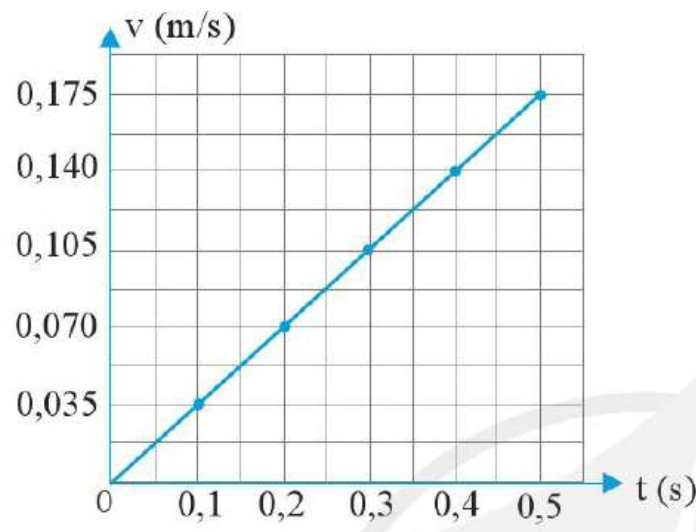
\includegraphics[scale=0.5]{figs/G10Y25B6-4}
		\captionof{figure}{Đồ thị vận tốc - thời gian}
		\label{fig:8.1}
	\end{center}
	Độ dốc của đồ thị $v$ - $t$ cho ta biết độ thay đổi vận tốc của vật theo thời gian, đồ thị càng dốc thì sự thay đổi vận tốc của vật diễn ra càng nhanh.\\
	Nếu vật chuyển động thẳng đều thì vận tốc không thay đổi theo thời gian, đồ thị vận tốc - thời gian là một đường thẳng song song với trục hoành $Ot$.
	\begin{center}
		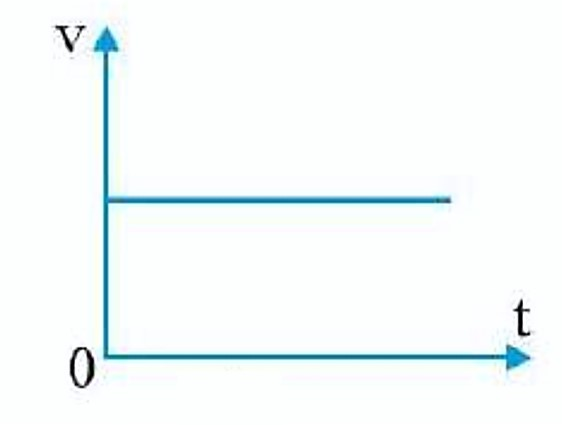
\includegraphics[scale=0.4]{figs/G10Y25B6-3}
		\captionof{figure}{Đồ thị vận tốc - thời gian của vật chuyển động thẳng đều.}
	\end{center}
	\paragraph{Gia tốc}
	Gia tốc là đại lượng đặc trưng cho độ biến thiên của vận tốc theo thời gian. Trong chuyển động thẳng, gia tốc trung bình được xác định theo biểu thức:
	$$a_\text{tb}=\dfrac{\Delta v}{\Delta t}=\dfrac{v_2-v_1}{\Delta t}$$
	Gia tốc tức thời tại một thời điểm có giá trị bằng độ dốc của tiếp tuyến của đồ thị vận tốc - thời gian $\left(v - t\right)$ tại thời điểm đó.
	\begin{center}
		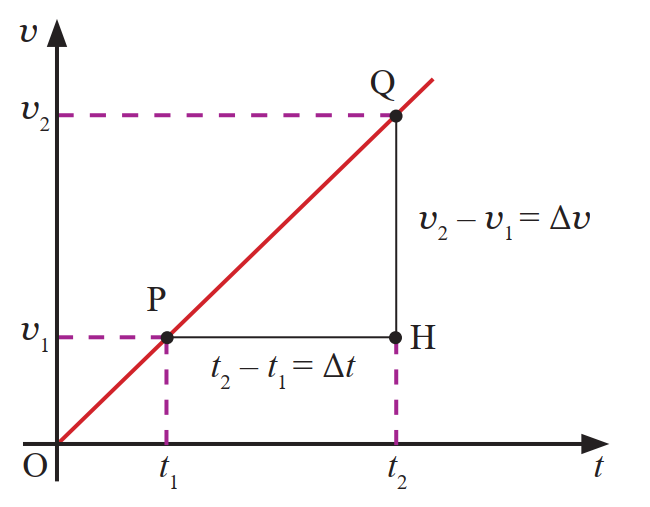
\includegraphics[scale=0.6]{figs/G10Y25B6-2}
		\captionof{figure}{Minh hoạ cách xác định gia tốc từ đồ thị vận tốc - thời gian.}
		\label{fig:8.2}
	\end{center}
	Trong hệ SI, gia tốc có đơn vị là $\si{\meter/\second^2}$.
	\paragraph{Vectơ gia tốc}
	Do vận tốc là một đại lượng vectơ nên gia tốc cũng là một đại lượng vectơ. Vectơ gia tốc trung bình được xác định:
	$$\overrightarrow{a_\text{tb}}=\dfrac{\Delta \vec{v}}{\Delta t}=\dfrac{\overrightarrow{v_2}-\overrightarrow{v_1}}{\Delta t}$$
	Khi $\Delta t$ rất nhỏ, gia tốc trung bình trở thành gia tốc tức thời có:
	\begin{itemize}
		\item gốc tại vị trí của vật;
		\item hướng cùng hướng với độ biến thiên vận tốc $\Delta \vec{v}$;
		\item độ dài tỉ lệ với độ lớn của vectơ $\Delta \vec{v}$ theo một tỉ xích xác định.
	\end{itemize}
	Gia tốc tức thời có thể được đo bằng gia tốc kế.
	\subsubsection{Phân biệt một số loại chuyển động thẳng}
	\begin{center}
		\begin{tabular}{|m{4cm}|m{6cm}|m{7cm}|}
			\hline
			\thead{$a=0$} & \thead{$a\neq 0$ và bằng hằng số} & \thead{$a\neq 0$ nhưng không phải hằng số}\\
			\hline
			chuyển động thẳng đều, vật có độ lớn vận tốc không đổi. & chuyển động thẳng biến đổi đều, vật có độ lớn vận tốc thay đổi (tăng hoặc giảm) đều theo thời gian. & chuyển động thẳng biến đổi phức tạp.\\
			\hline
		\end{tabular}
	\end{center}
	\paragraph{Vận dụng đồ thị $(v - t)$ để xác định độ dịch chuyển}
	Độ dịch chuyển của vật trong khoảng thời gian từ $t_1$ đến $t_2$ được xác định bằng phần diện tích giới hạn bởi các đường $v\left(t\right)$, $v=0$, $t=t_1$, $t=t_2$ trong đồ thị $\left(v - t\right)$.\\
	\textbf{\textit{Ví dụ:}} Xét vật chuyển động thẳng nhanh dần đều có vận tốc $v_1$ vào thời điểm $t_1=0$ và vận tốc $v_2$ tại thời điểm $t_2$. Độ dịch chuyển của vật trong khoảng thời gian $\Delta t= t_2-t_1$ chính là phần diện tích hình thang $OABD$ trong Hình \ref{fig:8.4}.
	\begin{center}
		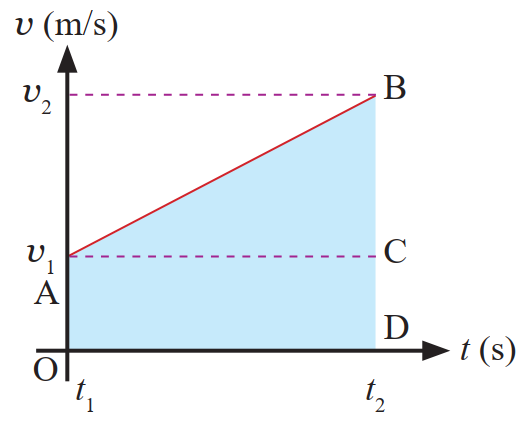
\includegraphics[scale=0.5]{figs/G10Y25B6-1}
		\captionof{figure}{Đồ thị $\left(v - t\right)$ của vật chuyển động thẳng biến đổi đều.}
		\label{fig:8.4}
	\end{center}
\subsubsection{Chuyển động thẳng biến đổi đều}

Chuyển động thẳng biến đổi đều là chuyển động có 
\begin{itemize}
	\item quỹ đạo là đường thẳng
	\item độ lớn của vận tốc tức thời tăng đều hoặc giảm đều theo thời gian.
\end{itemize}  
\begin{center}
	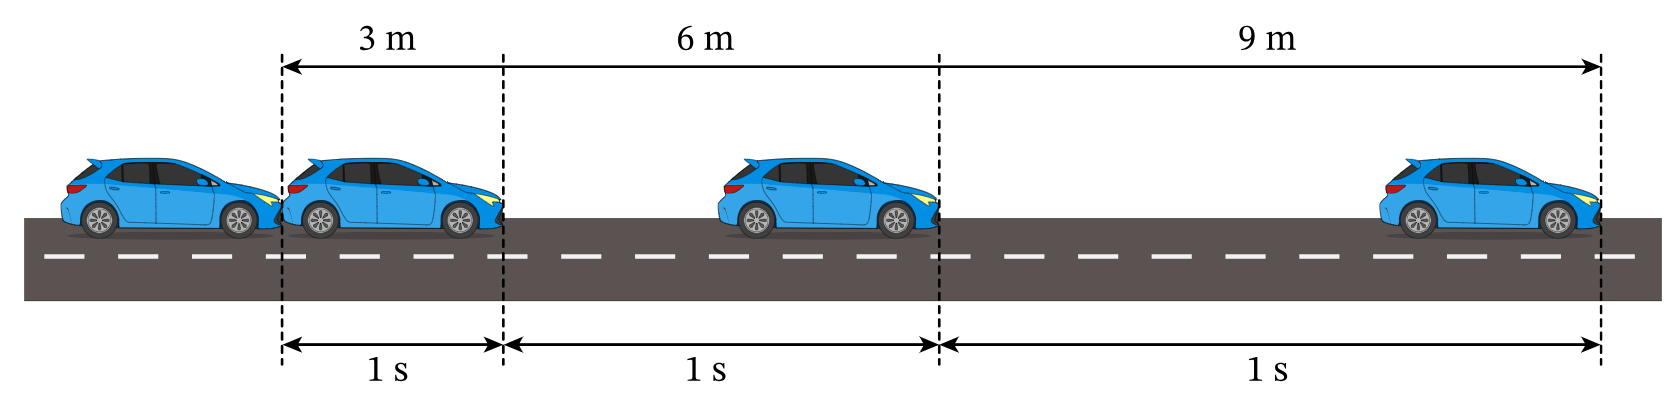
\includegraphics[scale=0.5]{figs/G10Y25B6-9}
	\captionof{figure}{Minh hoạ chuyển động thẳng biến đổi đều của một ô tô với gia tốc $\SI{3}{\meter/\second^2}$.}
\end{center}
\begin{center}
	\begin{tabular}{|m{20em}|m{20em}|}
		\hline
		\thead{Chuyển động thẳng nhanh dần đều} & \thead{Chuyển động thẳng chậm dần đều}\\
		\hline
		Tốc độ tăng đều theo thời gian & Tốc độ giảm đều theo thời gian\\
		$\vec{a}$ và $\vec{v}$ cùng chiều, $a\cdot v>0$ & $\vec{a}$ và $\vec{v}$ ngược chiều, $a\cdot v<0$\\
		\hline
	\end{tabular}
\end{center}
\subsubsection{Các phương trình của chuyển động thẳng biến đổi đều}
\paragraph{Phương trình gia tốc}
$$a=\text{hằng số}$$
\begin{luuy}
	Nếu chọn chiều chuyển động là chiều dương
	\begin{itemize}
		\item $a>0$: vật chuyển động nhanh dần đều.
		\item $a<0$: vật chuyển động chậm dần đều.
	\end{itemize}
\end{luuy}
\paragraph{Phương trình vận tốc}
Xét tại thời điểm $t_0=0$, vật chuyển động với vận tốc $v_0$ và gia tốc $a$. Tại thời điểm $t$, vật có vận tốc 
\begin{equation}
	v=v_0+at,
\end{equation}
Trong chuyển động thẳng biến đổi đều gia tốc $a$ có giá trị không đổi, vận tốc tức thời $v$ là hàm bậc nhất theo $t$ nên đồ thị vận tốc - thời gian có dạng là một nửa đường thẳng.
\begin{center}
	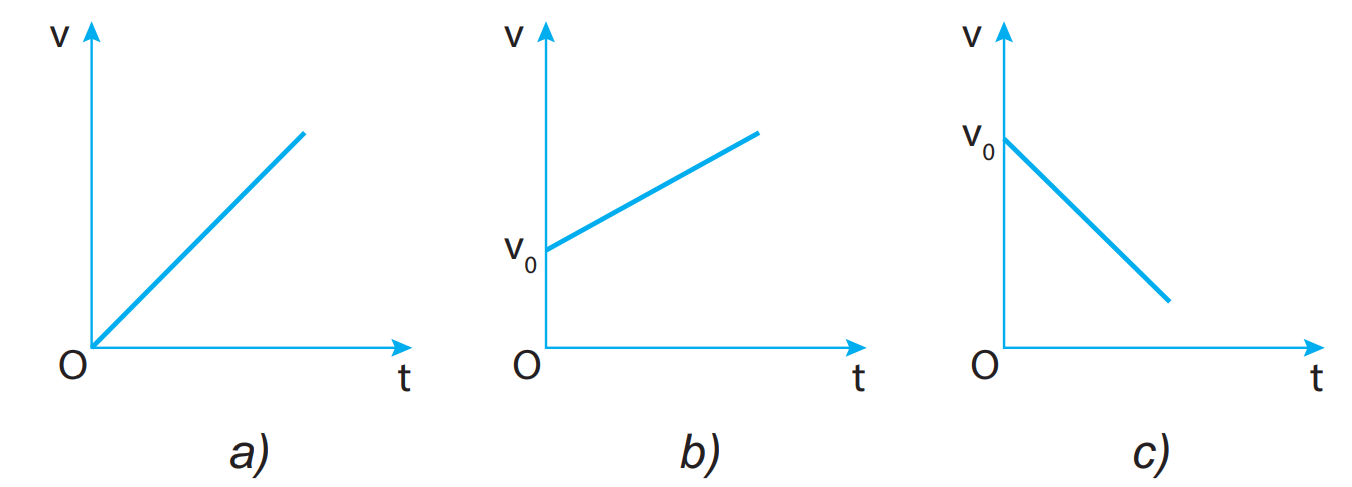
\includegraphics[scale=0.4]{figs/G10Y25B6-12}
	\captionof{figure}{Đồ thị vận tốc - thời gian của vật chuyển động thẳng biến đổi đều.
		\textit{Hình a)} Vật chuyển động nhanh dần đều từ trạng thái nghỉ; \textit{Hình b)} Vật chuyển động thẳng nhanh dần đều, \textit{Hình c)} Vật chuyển động thẳng chậm dần đều.}
\end{center}
Nếu trong quá trình chuyển động vật có đổi chiều chuyển động thì đồ thị vận tốc - thời gian có dạng:\\
\begin{minipage}[l]{10cm}
	\begin{center}
		\begin{tikzpicture}
			\coordinate (O) at (0,0);
			\coordinate (xaxis) at (5,0);
			\coordinate (ydaxis) at (0,-2);
			\coordinate (yuaxis) at (0,2);
			\draw[->,name path=Ox] (O)--(xaxis);
			\draw[->,name path=Oy] (ydaxis)--(yuaxis);
			\node[below left] at (O) {O};
			\node[above left] at (yuaxis) {$v$ };
			\node[right] at (xaxis) {$t$ };
			\path (0,-1.5) coordinate (vo) node[left] {$v_0$};
			\path (4,1.5) coordinate (v) node[left] {};
			\draw[thick,blue,name path=line] (vo)--(v);
			\node[above,text width=2.5cm,align=center] (1) at (2,1.5) {\small{nhanh dần đều }\\$a\cdot v>0$};
			\draw[->] (1.south) to [bend right] (2.7,0.8);
			\node[below,text width=1.5cm,align=center] (2) at (3.5,0) {\small{dừng lại}\\$v=0$};
			\path [name intersections={of=Ox and line,by=E}];
			\filldraw[red] (E) circle (2pt);
			\draw[->] (2.west) to [bend left] (2.05,-0.1);
			\node[below,text width=2.5cm,align=center] (3) at (3.5,-1.5) {\small{chậm dần đều}\\$a\cdot v<0$};
			\draw[->] (3.west) to [bend left] (1,-1);
		\end{tikzpicture}
		\captionof{figure}{Đồ thị hướng lên trên: $a>0$}
	\end{center}
\end{minipage}
\begin{minipage}[l]{10cm}
	\begin{center}
		\begin{tikzpicture}
			\coordinate (O) at (0,0);
			\coordinate (xaxis) at (5,0);
			\coordinate (ydaxis) at (0,-2);
			\coordinate (yuaxis) at (0,2);
			\draw[->,name path=Ox] (O)--(xaxis);
			\draw[->,name path=Oy] (ydaxis)--(yuaxis);
			\node[below left] at (O) {O};
			\node[above left] at (yuaxis) {$v$ };
			\node[right] at (xaxis) {$t$ };
			\path (0,1.5) coordinate (vo) node[left] {$v_0$};
			\path (4,-1.5) coordinate (v) node[left] {};
			\draw[thick,blue,name path=line] (vo)--(v);
			\node[above,text width=2.5cm,align=center] (1) at (2.5,1.5) {\small{chậm dần đều }\\$a\cdot v<0$};
			\draw[->] (1.south) to [bend left] (1.2,0.8);
			\node[below,text width=1.2cm,align=center] (2) at (0.8,0) {\small{dừng lại}\\$v=0$};
			\path [name intersections={of=Ox and line,by=E}];
			\filldraw[red] (E) circle (2pt);
			\draw[->] (2.east) to [bend right] (2,-0.1);
			\node[below,text width=2.5cm,align=center] (3) at (1.2,-1.5) {\small{nhanh dần đều}\\$a\cdot v>0$};
			\draw[->] (3.east) to [bend right] (3,-1);
		\end{tikzpicture}
		\captionof{figure}{Đồ thị hướng xuống dưới: $a<0$}
	\end{center}
\end{minipage}
\subsubsection{Phương trình độ dịch chuyển}
\begin{center}
	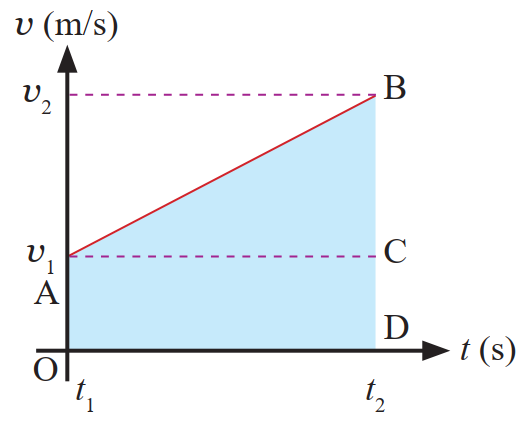
\includegraphics[scale=0.4]{figs/G10Y25B6-10}
	\captionof{figure}{Đồ thị $\left(v - t\right)$ của vật chuyển động thẳng biến đổi đều.}
	\label{fig:9.3}
\end{center}
Dựa vào đồ thị $\left(v - t\right)$ Hình \ref{fig:9.3} của vật chuyển động thẳng biến đổi đều. Ta có độ dịch chuyển trong khoảng thời gian $\Delta t= t- 0 =t$ chính là diện tích hình thang $OABD$:
$$d=\dfrac{1}{2}\left(OA+BD\right)\cdot OD=\dfrac{1}{2}\left(v+v_0\right)\cdot t$$
Mà $v=v_0+at$
Ta rút ra được phương trình độ dịch chuyển của vật:
$$d=v_0\cdot t+\dfrac{1}{2}a\cdot t^2$$
Đồ thị $\left(d - t\right)$ của chuyển động thẳng biến đổi đều được biểu diễn trong Hình \ref{fig:9.4} là một nhánh parabol.
\begin{center}
	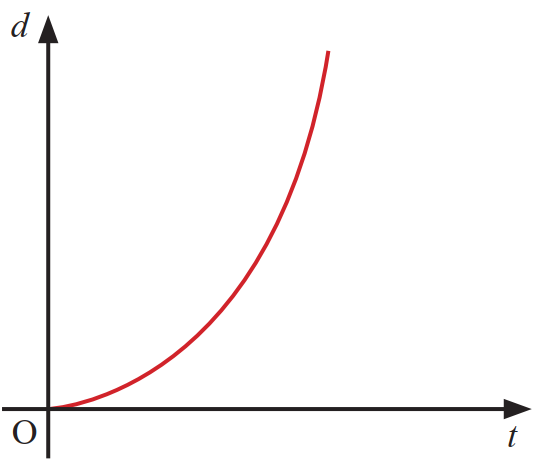
\includegraphics[scale=0.5]{figs/G10Y25B6-11}
	\captionof{figure}{Đồ thị $\left(d - t\right)$ của vật chuyển động thẳng biến đổi đều.}
	\label{fig:9.4}
\end{center}
Nếu tại thời điểm $t_0$, vật ở vị trí $x_0$ so với gốc toạ độ. Do $d=x-x_0$, ta rút ra được phương trình xác định toạ độ của vật chuyển động thẳng biến đổi đều
$$x=x_0+v_0\cdot t+\dfrac{1}{2}a\cdot t^2$$
trong đó:
\begin{itemize}[label=$\circ$]
	\item $x_0$: tọa độ ban đầu của vật tại thời điểm $t_0$;
	\item $x$: tọa độ của vật tại thời điểm $t$;
	\item $v_0$: vận tốc của vật ($v_0>0$ nếu vật chuyển động cùng chiều dương, $v_0<0$ nếu vật chuyển động ngược chiều dương);
	\item $a$: gia tốc của vật ($a\cdot v_0>0$ nếu vật chuyển động nhanh dần đều, $a\cdot v_0<0$ nếu vật chuyển động chậm dần đều).
\end{itemize}
\subsubsection{Phương trình liên hệ giữa gia tốc, vận tốc và độ dịch chuyển}
$$v^2-v^2_0=2a\cdot d$$

\subsubsection{Phương trình toạ độ của chất điểm chuyển động thẳng biến đổi đều}
Phương trình chuyển động của vật là phương trình mô tả sự thay đổi tọa độ của vật theo thời gian. \\
Để lập phương trình toạ độ của vật chuyển động thẳng biến đổi đều, ta thực hiện các bước như sau:
\begin{itemize}
	\item Chọn hệ quy chiếu gồm:
	\begin{itemize}
		\item Gốc tọa độ (thường là vị trí xuất phát của một vật);
		\item Mốc thời gian (thường là thời điểm bắt đầu chuyển động của một vật);
		\item Chiều dương (thường là chiều chuyển động của một vật).
	\end{itemize}
	\item Xét một điểm chuyển động thẳng biến đổi đều trên đường thẳng O$x$. Ở thời điểm ban đầu ($t_0$), chất điểm ở vị trí A có tọa độ $x_{0}$  với vận tốc ban đầu $v_0$ và gia tốc $a$. Mốc thời gian được chọn lúc bắt đầu chuyển động. Ở thời điểm $t$, chất điểm ở vị trí B có tọa độ $x$ như hình vẽ.  	
	\begin{center}
		\begin{tikzpicture}
			\coordinate (laxis) at (-0.5,0);
			\coordinate (O) at (0,0);
			\coordinate (A) at (2,0);
			\coordinate (va) at ($(A)+(1,0)$);
			\coordinate (raxis) at (8,0);
			\coordinate (ldaxis) at (-0.5,-1);
			\coordinate (Od) at (0,-1);
			\coordinate (Ad) at (2,0);
			\coordinate (B) at (5,-1);
			\coordinate (vb) at ($(B)+(2,0)$);
			\coordinate (rdaxis) at (8,-1);
			\draw[->] (laxis) -- (raxis);
			\draw[->] (ldaxis) -- (rdaxis);
			
			
			\draw[->,ultra thick,blue] (A) -- (va);
			\draw[->,ultra thick,green!60!black] (B) -- (vb);
			\node[above=2mm] at (A) {A};
			\node[below left=1mm and 0.5mm] at (A) {$x_0$};
			\node[above=2mm] at (B) {B};
			\node[below left=1mm and 0.5mm] at (B) {$x$};
			\node[above=2mm] at (O) {O};
			
			%		\node[above=2mm] at (Od) {O};
			%		\node[below=2mm] at (C) {C};
			\node[right] at (raxis) {$x$};
			\node[above=1mm] at (va) {$\vec{v}_{0}$};
			\node[above=1mm] at (vb) {$\vec{v}$};
			
			\node[left=3cm,anchor=west] at (laxis) {thời điểm $t_0$};
			\node[left=3cm,anchor=west] at (ldaxis) {thời điểm $t> t_0$};
			\foreach \i in {O,Od,B,A}
			{
				\filldraw (\i) circle (2pt);
			}
			
			%		\coordinate (odd) at ($(O)-(0,2)$);
			\coordinate (add) at ($(A)-(0,2)$);
			\coordinate (bdd) at ($(B)-(0,1)$);
			%		\draw[<->,thick] (odd) -- (add);
			
			\draw[dashed] (O)--(Od);
			\draw[<->] (add) -- (bdd) node[midway,fill= white] {$d$};
			\draw[dashed] (A)--(add);
			\draw[dashed] (B)--(bdd);
			
		\end{tikzpicture}
	\end{center}
	Phương trình chuyển động của vật có dạng tổng quát như sau:
	\begin{equation*}
		x=x_0+d=x_0+v_0\cdot(t-t_0)+\dfrac{1}{2}a\cdot(t-t_0)^2\qquad\textrm{ với }(t\geq t_0),
	\end{equation*}
	Thông thường, để thuận tiện trong tính toán, ta chọn thời điểm $t_0=0$, khi đó phương trình chuyển động của chất điểm trở thành 
	\begin{equation*}
		x=x_0+v_0t+\dfrac{1}{2}at^{2}.
	\end{equation*}
\end{itemize}	
\subsubsection{Điều kiện để hai vật gặp nhau}
Hai vật gặp nhau khi chúng có cùng tọa độ:
\begin{equation*}
	x_1=x_2.
\end{equation*}
\subsubsection{Khoảng cách giữa hai vật trong quá trình chuyển động}
Khoảng cách giữa hai vật tại thời điểm $t$ bất kì là:
\begin{equation*}
	\Delta x=\left|x_1-x_2\right|.
\end{equation*}
\end{tomtat}
\subsection{VÍ DỤ MINH HỌA}
\begin{dang}{Phân biệt một số loại chuyển động thẳng }
\end{dang}
\begin{vd}
	Trong các chuyển động sau đây, chuyển động nào có giá trị gia tốc không phải là một hằng số trong suốt quá trình chuyển động?
	\begin{enumerate}[label=\alph*)]
		\item Một người đi xe đạp đang tăng tốc đều trên đường thẳng từ trạng thái đứng yên.
		\item Một quả bóng nằm yên trên bàn.
		\item Một thang máy chuyển động từ tầng 2 lên tầng 4 và có dừng đón khách tại tầng 3?
	\end{enumerate}
	Hãy giải thích các câu trả lời mà em đưa ra.
	\loigiai{
		\begin{enumerate}[label=\alph*)]
			\item Người đi xe đạp có gia tốc là một hằng số vì xe được tăng tốc đều.
			\item Quả bóng có gia tốc là một hằng số (bằng 0) vì quả bóng không thay đổi trạng thái chuyển động.
			\item Thang máy có gia tốc không phải là một hằng số vì có lúc chuyển động nhanh dần, có lúc chuyển động chậm dần.
		\end{enumerate}
	}
\end{vd}

\begin{vd}
	Hình \ref{fig:8.8} là đồ thị vận tốc - thời gian trong chuyển động của một bạn đang đi trong siêu thị. Hãy dựa vào đồ thị để mô tả bằng lời chuyển động của bạn đó (khi nào đi đều, đi nhanh lên, đi chậm lại, nghỉ).
	\begin{center}
		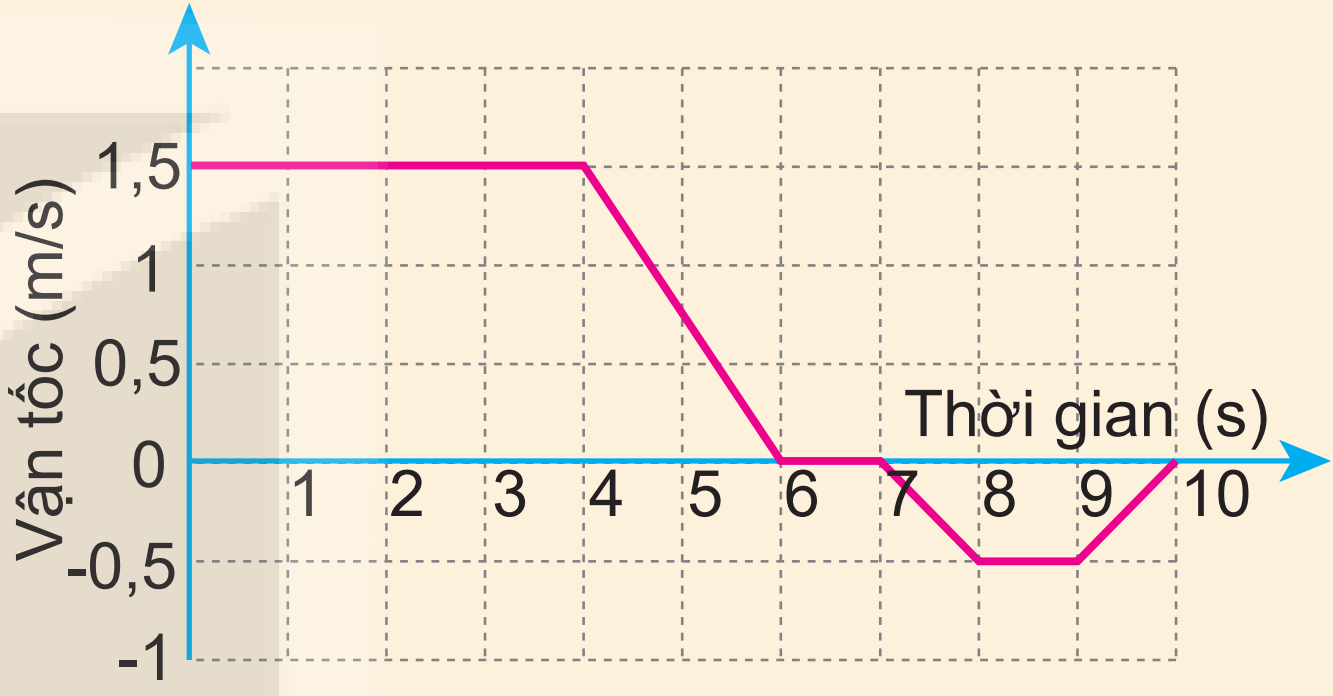
\includegraphics[scale=0.3]{figs/G10Y25B6-5}
		\captionof{figure}{Đồ thị $\left(v - t\right)$ của bạn đang đi trong siêu thị.}
		\label{fig:8.8}
	\end{center}
	\loigiai{
		Mô tả chuyển động của bạn này:
		\begin{itemize}
			\item Trong $\SI{4}{\second}$ đầu tiên: bạn đi đều với tốc độ $\SI{1.5}{\meter/\second}$.
			\item Từ thời điểm $\SI{4}{\second}$ đến $\SI{6}{\second}$: bạn đi chậm lại.
			\item Từ thời điểm $\SI{6}{\second}$ đến $\SI{7}{\second}$: bạn đứng yên.
			\item Từ thời điểm $\SI{7}{\second}$ đến thời điểm $\SI{8}{\second}$: bạn đổi chiều chuyển động và đi nhanh dần theo chiều âm.
			\item Từ thời điểm $\SI{8}{\second}$ đến thời điểm $\SI{9}{\second}$: bạn đi đều với tốc độ $\SI{0.5}{\meter/\second}$ theo chiều âm.
			\item Từ thời điểm $\SI{9}{\second}$ đến thời điểm $\SI{10}{\second}$: bạn đi chậm dần theo chiều âm và dừng lại tại thời điểm $\SI{10}{\second}$.
		\end{itemize}
	}
\end{vd}
\begin{dang}{Vẽ được đồ thị vận tốc – thời gian trong chuyển động thẳng}
\end{dang}
\begin{vd}
	Một người lái xe tải đang cho xe chạy trên đường cao tốc với vận tốc không đổi. Khi thấy khoảng cách giữa xe mình với xe chạy phía trước giảm dần, người đó cho xe chạy chậm dần. Tới khi thấy khoảng cách này đột nhiên giảm nhanh, người đó vội đạp phanh để dừng xe. Hãy vẽ đồ thị vận tốc - thời gian mô tả trạng thái chuyển động của xe tải trên.
	\loigiai{
		Chuyển động xe tải qua 3 giai đoạn:
		\begin{itemize}
			\item Giai đoạn từ ban đầu đến thời điểm $t_1$ xe chuyển động với vận tốc không đổi. Đồ thị $\left(v - t\right)$ là một đoạn thẳng song song với trục $Ot$.
			\item Giai đoạn 2 từ thời điểm $t_1$ đến thời điểm $t_2$: xe giảm tốc dần. Đồ thị $\left(v - t\right)$ có hệ số góc âm.
			\item Giai đoạn 3 từ thời điểm $t_2$ đến thời điểm $t_3$: xe giảm tốc nhanh về 0.
		\end{itemize}
		\begin{center}
			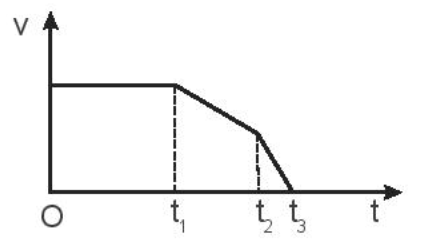
\includegraphics[scale=0.7]{figs/G10Y25B6-6}
			\captionof{figure}{Đồ thị vận tốc - thời gian của xe tải.}
		\end{center}
	}
\end{vd}

\begin{vd}
	Xét một vận động viên chạy xe đạp trên một đoạn đường thẳng. Vận tốc của vận động viên này tại mỗi thời điểm được ghi lại trong bảng dưới đây.
	\begin{center}
		\begin{tabular}{|c|ccccccccccc|}
			\hline
			$t \left(\si{\second}\right)$ & 0 & 5 & 10 & 15 &20 & 25 & 30 & 35 & 40 & 45 & 50\\
			\hline
			$v \left(\si{\meter/\second}\right)$ & 5 & 5 & 8 & 9 & 10 & 10 & 10 & 12 & 14 & 16 & 16 \\
			\hline
		\end{tabular}
	\end{center}
	Hãy vẽ đồ thị vận tốc – thời gian và mô tả tính chất chuyển động của vận động viên này.
	\loigiai{
		\begin{center}
			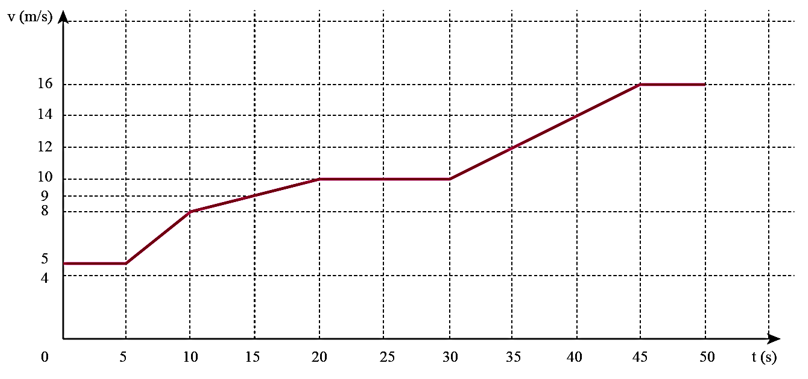
\includegraphics[scale=0.7]{figs/G10Y25B6-7}
			\captionof{figure}{Đồ thị vận tốc - thời gian của vận động viên.}
		\end{center}
		Tính chất chuyển động của vận động viên:
		\begin{itemize}
			\item Trong $\SI{5}{\second}$ đầu: chuyển động thẳng đều với vận tốc $\SI{5}{\meter/\second}$.
			\item Trong $\SI{5}{\second}$ tiếp theo: chuyển động thẳng nhanh dần đều với gia tốc $\SI{0.6}{\meter/\second^2}$.
			\item Từ thời điểm $\SI{10}{\second}$ đến thời điểm $\SI{20}{\second}$: chuyển động thẳng nhanh dần đều với gia tốc $\SI{0.2}{\meter/\second^2}$.
			\item Từ thời điểm $\SI{20}{\second}$ đến thời điểm $\SI{30}{\second}$: chuyển động thẳng đều với vận tốc $\SI{10}{\meter/\second}$.
			\item Trong $\SI{15}{\second}$ kế tiếp: chuyển động thẳng nhanh dần đều với gia tốc $\SI{0.4}{\meter/\second^2}$.
			\item Sau đó, vận động viên chuyển động thẳng đều với vận tốc $\SI{16}{\meter/\second}$.
		\end{itemize}
	}
\end{vd}
\begin{dang}{Vận dụng đồ thị vận tốc – thời gian để tính được độ dịch chuyển và gia tốc trong một số trường hợp đơn giản}
\end{dang}
\begin{vd}
	Dựa vào đồ thị $\left(v - t\right)$ của vật chuyển động trong Hình \ref{fig:8.7}, hãy xác định gia tốc và độ dịch chuyển của vật trong các giai đoạn:
	\begin{center}
		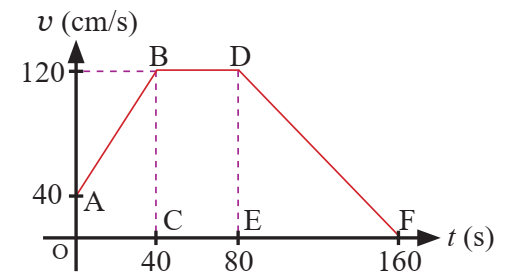
\includegraphics[scale=0.6]{figs/G10Y25B6-8}
		\captionof{figure}{Đồ thị $\left(v - t\right)$ của một vật chuyển động.}
		\label{fig:8.7}
	\end{center}
	\begin{enumerate}[label=\alph*)]
		\item Từ $\SI{0}{\second}$ đến $\SI{40}{\second}$.
		\item Từ $\SI{80}{\second}$ đến $\SI{160}{\second}$.
	\end{enumerate}
	\loigiai{
		Chọn chiều dương là chiều chuyển động của vật.\\
		Gia tốc và độ dịch chuyển của vật trong các giai đoạn:
		\begin{enumerate}[label=\alph*)]
			\item $a_1=\dfrac{v_B-v_A}{t_B-t_A}=\dfrac{\left(\SI{120}{\centi\meter/\second}\right)-\left(\SI{40}{\centi\meter/\second}\right)}{\SI{40}{\second}}=\SI{2}{\centi\meter/\second^2}$.\\
			$d_1=\dfrac{1}{2}\cdot\left(OA+BC\right)\cdot OC=\dfrac{1}{2}\cdot\left(\SI{160}{\centi\meter/\second}\right)\cdot \left(\SI{40}{\second}\right)=\SI{3200}{\centi\meter}$.
			\item Tương tự câu a, ta có:
			$a_2 =\dfrac{v_F-v_D}{t_F - t_D}=\dfrac{\left(\SI{0}{\centi\meter/\second}\right)-\left(\SI{120}{\centi\meter/\second}\right)}{\left(\SI{160}{\second}\right)-\left(\SI{80}{\second}\right)}=\SI{-1.5}{\centi\meter/\second^2}$\\
			$d_2=\dfrac{1}{2}\cdot ED \cdot EF=\dfrac{1}{2}\cdot\left(\SI{120}{\centi\meter/\second}\right)\cdot\left(\SI{160}{\second}-\SI{80}{\second}\right)=\SI{4800}{\centi\meter}$.
		\end{enumerate}
	}
\end{vd}
\begin{dang}{Nhận biết được đặc điểm \\của chuyển động thẳng biến đổi đều}
\end{dang}
\begin{vd}
	Chuyển động thẳng biến đổi đều là chuyển động
	\choice
	{có quỹ đạo là đường thẳng, vectơ gia tốc bằng không.}
	{\True có quỹ đạo là đường thẳng, vectơ gia tốc không thay đổi trong suốt quá trình chuyển động.}
	{có quỹ đạo là đường thẳng, vectơ gia tốc và vận tốc không thay đổi trong suốt quá trình chuyển động.}
	{có quỹ đạo là đường thẳng, vectơ vận tốc không thay đổi trong suốt quá trình chuyển động.}
	\loigiai{
		Chuyển động thẳng biến đổi đều là chuyển động có quỹ đạo là đường thẳng, vectơ gia tốc không thay đổi trong suốt quá trình chuyển động.
	}
\end{vd}

\begin{vd}
	Đồ thị nào sau đây là của chuyển động thẳng biến đổi?
	\begin{center}
		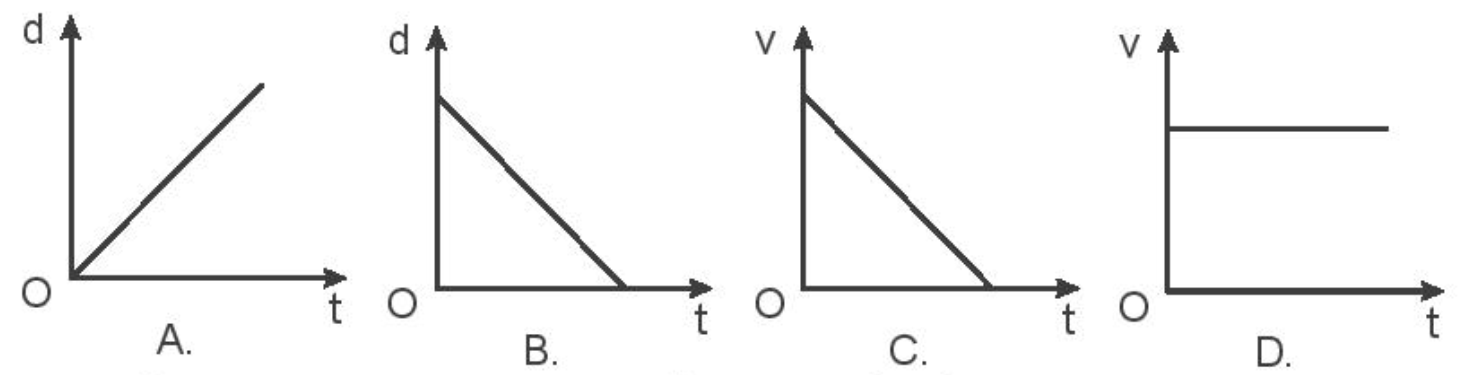
\includegraphics[scale=0.5]{figs/G10Y25B6-13}
	\end{center}
	\loigiai{
		Hình a) và b): Đồ thị $\left(d - t\right)$ là một đường thẳng thay đổi theo $t$, do đó đây là chuyển động thẳng đều.\\
		Hình d): Đồ thị $\left( v - t\right)$ là một đường thẳng song song với trục $Ot$. Do đó, vận tốc không thay đổi theo thời gian. Đây là chuyển động thẳng đều.\\
		Hình c): Đồ thị $\left(v - t\right)$ là có dạng đường thẳng thay đổi theo $t$. Do đó, vận tốc là hàm bậc nhất của thời gian. Đây là chuyển động thẳng biến đổi đều.
	}
\end{vd}
\begin{dang}{Áp dụng được công thức liên hệ giữa độ dời, vận tốc, gia tốc }
\end{dang}
\begin{vd}
	Một xe máy đang đi với $v = \SI{50.4}{\kilo\meter/\hour}$ bỗng người lái xe thấy có ổ gà trước mắt cách xe $\SI{24.5}{\meter}$. Người ấy phanh gấp và xe đến ổ gà thì dừng lại.
	\begin{enumerate}[label=\alph*)]
		\item Tính gia tốc.
		\item Tính thời gian phanh.
	\end{enumerate}
	\loigiai{
		Đơn vị vận tốc được đổi về hệ SI $$\SI{50.4}{\kilo\meter/\hour} =\dfrac{\SI{50.4e3}{\meter}}{\SI{3600}{\second}}= \SI{14}{\meter/\second}.$$
		\begin{enumerate}[label=\alph*)]
			\item Gia tốc của xe máy
			$$v^2-v_0^2 =2a\cdot d \Rightarrow a =\dfrac{v^2 - v_0^2}{2d}=\dfrac{\left(\SI{0}{\meter/\second}\right)^{2}-\left(\SI{14}{\meter/\second}\right)^{2}}{2\cdot\SI{24.5}{\meter}}=\SI{-4}{\meter/\second^2}.$$
			\item Thời gian phanh
			
			$$v =v_0 +at \Rightarrow t = \dfrac{v-v_0}{a} =\dfrac{\SI{0}{\meter/\second}-\SI{14}{\meter/\second}}{\SI{-4}{\meter/\second^{2}}}= \SI{3.5}{\second}.$$
		\end{enumerate}
	}
\end{vd}

\begin{vd}
	Một đoàn tàu bắt đầu chuyển động nhanh dần đều khi đi hết $\SI{1}{\kilo\meter}$ đầu tiên thì đạt vận tốc $v=\SI{10}{\meter/\second}$. Tính vận tốc đoàn tàu sau khi đi hết $\SI{2}{\kilo\meter}$.
	\loigiai{
		Gia tốc của đoàn tàu
		$$v^2-v_0^2 =2a\cdot d_1 \Rightarrow a = \dfrac{v^2-v_0^2}{2d_1}=\dfrac{\left(\SI{10}{\meter/\second}\right)^2-(\SI{0}{\meter/\second})^2}{2\cdot\SI{1000}{\meter}} =\SI{0.05}{\meter/\second^2}.$$
		
		Vận tốc sau khi đi hết $\SI{2}{\kilo\meter}$
		$$v_1^2 - v_0^2 = 2a\cdot d_2 \Rightarrow  v_1 =\sqrt{2ad_2+v_0^2}=\sqrt{2\cdot\SI{0.05}{\meter/\second^{2}}\cdot\SI{2000}{\meter}+\left(\SI{0}{\meter/\second}\right)^{2}} =\xsi{10\sqrt{2}}{\meter/\second}.$$
	}
\end{vd}
\begin{dang}{Xây dựng đồ thị vận tốc - thời gian của vật chuyển động thẳng biến đổi đều}
\end{dang}
\begin{vd}
	Một vật chuyển động có đồ thị vận tốc như hình vẽ. Công thức vận tốc và công thức đường đi của vật là
	\begin{center}
		\begin{tikzpicture}
			\coordinate (O) at (0,0);
			\coordinate (xaxis) at (3.5,0);
			\coordinate (yaxis) at (0,3);
			\draw[->] (O)--(xaxis);
			\draw[->] (O)--(yaxis);
			\node[below left] at (O) {O};
			\node[above] at (yaxis) {$v$ (\si{\meter/\second})};
			\node[right] at (xaxis) {$t$ (\si{\second})};
			\path (0,1) coordinate (vo) node[left] {20};
			\coordinate (v) at ($(vo)+(30:3)$);
			\coordinate (vt) at ($(vo)+(30:2)$);
			\draw[thick,blue] (vo)--(v);
			\path let \p1=(vt) in (\x1,0) coordinate (vtx) node[below] {20};
			\path let \p1=(vt) in (0,\y1) coordinate (vty) node[left] {40};
			\draw[dashed] (vt)--(vtx);
			\draw[dashed] (vt)--(vty);
		\end{tikzpicture}
	\end{center}
	\choice
	{$v=t$, $s=\dfrac{1}{2}t^2$.}
	{\True $v=20+t$, $s=20t+\dfrac{1}{2}t^2$.}
	{$v=20-t$, $s=20t-\dfrac{1}{2}t^2$.}
	{$v=40-2t$, $s=40t-\dfrac{1}{2}t^2$.}
	\loigiai{
		Đồ thị vận tốc - thời gian có dạng đường thẳng với hệ số góc khác không nên đây là đồ thị mô tả chuyển động thẳng biến đổi đều.
		
		Gia tốc của vật được tính theo công thức
		\begin{equation*}
			a=\dfrac{v-v_0}{t}=\dfrac{\SI{40}{\meter/\second}-\SI{20}{\meter/\second}}{\SI{20}{\second}}=\SI{1}{\meter/\second^2}.
		\end{equation*}
		
		Phương trình vận tốc có dạng
		\begin{equation*}
			v=v_0+at=20+t\textrm{ (\si{\meter/\second}, \si{\second})}.
		\end{equation*}
		
		Công thức tính quãng đường đi được
		\begin{equation*}
			s=v_0 t+\dfrac{1}{2}at^2=20t+\dfrac{1}{2}t^2\textrm{ (\si{\meter}, \si{\second})}.
		\end{equation*}
	}
\end{vd}

\begin{vd}
	Một xe đạp đang chuyển động với vận tốc $\SI{5}{\meter/\second}$ thì hãm phanh chuyển động chậm dần đều có đồ thị vận tốc theo thời gian sau. Tính quãng đường đi được từ lúc hãm phanh cho đến khi dừng lại.
	
	\begin{center}
		\begin{tikzpicture}
			\coordinate (O) at (0,0);
			\coordinate (xaxis) at (4,0);
			\coordinate (yaxis) at (0,3);
			\draw[->] (O)--(xaxis);
			\draw[->] (O)--(yaxis);
			\node[below left] at (O) {O};
			\node[above] at (yaxis) {$v$ (\si{\meter/\second})};
			\node[right] at (xaxis) {$t$ (\si{\second})};
			\path (0,2) coordinate (vo) node[left] {5};
			\path (3,0) coordinate (v) node[below] {10};
			\draw[thick,blue] (vo)--(v);
		\end{tikzpicture}
	\end{center}
	\loigiai{
		Gia tốc của vật là
		\begin{equation*}
			a=\dfrac{v-v_0}{t}=\dfrac{\SI{0}{\meter/\second}-\SI{5}{\meter/\second}}{\SI{10}{\second}}=-\SI{0.5}{\meter/\second^2}.
		\end{equation*}
		
		Quãng đường đi được từ lúc hãm phanh cho đến khi dừng lại là:
		\begin{equation*}
			v^2-v_0^2=2a\cdot d\quad\Rightarrow\quad  s=\dfrac{v^2-v_0^2}{2a}=\dfrac{(\SI{0}{\meter/\second})^{2}-(\SI{5}{\meter/\second})^2}{2\cdot (\SI{-0.5}{\meter/\second^2})}=\SI{25}{\meter}.
		\end{equation*}
	}
\end{vd}

\begin{vd}
	Đồ thị vận tốc thời gian của một vật chuyển động như hình vẽ bên.
	\begin{center}
		\begin{tikzpicture}[scale=0.7]
			\coordinate (O) at (0,0);
			\coordinate (xaxis) at (7,0);
			\coordinate (yaxis) at (0,4);
			\draw[->] (O)--(xaxis);
			\draw[->] (O)--(yaxis);
			\node[below left] at (O) {O};
			\node[left] at (yaxis) {$v$ (\si{\meter/\second})};
			\node[right] at (xaxis) {$t$ (\si{\second})};
			\coordinate (A) at (0,2);
			\coordinate (B) at (1,3);
			\coordinate (C) at (3,3);
			\coordinate (D) at (6,0);				
			\node[above] at (B) {B};
			\node[above] at (C) {C};
			\node[above right] at (D) {D};
			\node[right] at (A) {A};
			\draw[thick,blue] (A)--(B)--(C)--(D);
			\path let \p1=(B) in (\x1,0) coordinate (bd) node[below] {10};
			\path let \p2=(C) in (\x2,0) coordinate (cd) node[below] {30};
			\path let \p3=(B) in (0,\y3) coordinate (bl) node[left] {15};
			\node[left] at (A) {10};
			\node[below] at (D) {60};
			\draw[dashed] (B)--(bd);
			\draw[dashed] (C)--(cd);
			\draw[dashed] (B)--(bl);
		\end{tikzpicture}
	\end{center}
	\begin{enumerate}[label=\alph*)]
		\item Nêu tính chất chuyển động của mỗi giai đoạn.
		\item Lập phương trình vận tốc của mỗi giai đoạn.
	\end{enumerate}
	
	\loigiai{
		\begin{enumerate}[label=\alph*)]
			\item Tính chất chuyển động của mỗi giai đoạn:
			\begin{itemize}
				\item Trên đoạn $AB$: chuyển động nhanh dần đều do đồ thị thể hiện vận tốc tăng với hệ số góc không đổi.
				\item Trên đoạn $BC$: chuyển động thẳng đều do đồ thị thể hiện vận tốc không thay đổi theo thời gian.
				\item Trên đoạn $CD$: chuyển động chậm dần đều đến khi dừng lại do đồ thị thể hiện vận tốc giảm đều về 0.
			\end{itemize}
			\item Phương trình vận tốc của mỗi giai đoạn	
			\begin{align*}
				v_\text{AB}& = \xsi{10 +0.5\cdot t}{\meter/\second} &(\SI{0}{\second}\leq t \leq \SI{10}{\second}),\\
				v_\text{BC} &= \SI{15}{\meter/\second}.&(\SI{10}{\second}<t\leq \SI{30}{\second}),\\
				v_\text{CD} &= \xsi{15 - 0.5\cdot t}{\meter/\second} & (\SI{30}{\second} < t \leq \SI{60}{\second}).
			\end{align*}
		\end{enumerate}
		
	}
\end{vd}
\begin{dang}{Xác định quãng đường, vận tốc, gia tốc, thời gian \\thông qua phương trình chuyển động }
\end{dang}
\begin{vd}
	Một vật chuyển động có phương trình toạ độ theo thời gian: $x = 6t^2 - 18t + 12 \ (\text{\si{\centi\meter}, \si{\second}})$. Hãy xác định:
	\begin{enumerate}[label=\alph*)]
		\item Vận tốc đầu, gia tốc của chuyển động và cho biết tính chất của chuyển động.
		\item Vận tốc của vật ở thời điểm $t = \SI{2}{\second}$.
	\end{enumerate}
	\loigiai{
		\begin{enumerate}[label=\alph*)]
			\item Đối chiếu phương trình
			$$x = 6t^2 - 18t + 12 \ \si{\centi\meter}$$
			với phương trình chuyển động
			$$x=x_0+v_0t+\dfrac{1}{2}at^{2}$$
			ta suy ra
			$$v_0 = \SI{-18}{\centi\meter/\second};\qquad a =\SI{12}{\centi\meter/\second^{2}}.$$
			
			Vật chuyển động chậm dần đều do gia tốc và vận tốc trái dấu với nhau.
			\item Thay các giá trị vận tốc và gia tốc đã tìm được vào phương trình vận tốc, ta suy ra vận tốc của vật ở thời điểm $t=\SI{2}{\second}$
			$$v =v_0 +at =\SI{-18}{\centi\meter/\second}+\SI{12}{\centi\meter/\second^{2}}\cdot\SI{2}{\second}=\SI{6}{\centi\meter/\second}.$$
		\end{enumerate}
	}
\end{vd}

\begin{vd}
	Một vật chuyển động thẳng có phương trình toạ độ theo thời gian: $x = 4t^2 + 20t\ (\si{\meter})$. Xác định độ dịch chuyển của vật từ thời điểm $t_1 = \SI{2}{\second}$ đến thời điểm $t_2 = \SI{5}{\second}$.
	\loigiai{
		Vị trí của vật ở thời điểm $\SI{2}{\second}$
		
		$$x_1 = 4t_1^2 + 20t_1 =\SI{56}{\meter}.$$
		
		Vị trí của vật ở thời điểm $\SI{5}{\second}$
		
		$$x_2 = 4t_2^2 + 20t_2 =\SI{200}{\meter}.$$
		
		Độ dịch chuyển của vật trong thời gian từ $\SI{2}{\second}$ đến $\SI{5}{\second}$ là:
		$$d = x_2 - x_1 = \SI{144}{\meter}.$$
	}
\end{vd}

\begin{vd}
	Vật chuyển động thẳng có phương trình: $x = 2t^2 - 4t + 10$ (đơn vị của $x$ và $t$ lần lượt là \si{\meter} và \si{\second}). Vật sẽ dừng lại tại vị trí
	\choice
	{$\SI{6}{\meter}.$}
	{$\SI{4}{\meter}.$}
	{$\SI{10}{\meter}.$}
	{\True $\SI{8}{\meter}.$}
	\loigiai{
		Vật sẽ dừng lại khi vận tốc $v = 0$.
		
		Từ phương trình chuyển động ta suy ra các giá trị vận tốc ban đầu và gia tốc
		$$v_0=\SI{-4}{\meter/\second},	\qquad a=\SI{4}{\meter/\second^{2}}.$$
		
		Sử dụng phương trình vận tốc, ta suy ra thời điểm vật dừng lại
		\begin{align*}
			v=v_0+at=0 \quad\Rightarrow\quad t=-\dfrac{v_0}{a}=-\dfrac{\SI{-4}{\meter/\second}}{\SI{4}{\meter/\second^{2}}}=\SI{1}{\second}.
		\end{align*}		
		Thay $t =\SI{1}{\second}$ vào phương trình chuyển động ta được vị trí dừng lại của vật
		$$x = 2t^2 - 4t + 10=\SI{8}{\meter}.$$
	}
\end{vd}
\begin{dang}{Xây dựng phương trình chuyển động thẳng biến đổi đều}
\end{dang}
\begin{vd}
	Một vật chuyển động thẳng chậm dần đều với tốc độ ban đầu $\SI{3}{\meter/\second}$ và gia tốc có độ lớn $\SI{2}{\meter/\second^2}$. Biết thời điểm ban đầu vật ở gốc tọa độ và chuyển động ngược chiều dương của trục tọa độ. Viết phương trình chuyển động của vật.
	\loigiai{
		Chọn gốc thời gian là khi vật bắt đầu chuyển động.
		
		Vì vật chuyển động chậm dần đều ngược chiều dương nên
		\begin{equation*}
			\left\{
			\begin{array}{rcl}
				a\cdot v &<&0\\
				v &<& 0
			\end{array}
			\right.
			\quad
			\Rightarrow 
			\left\{
			\begin{array}{rcl}
				a &>& 0\\
				v &<& 0.
			\end{array}
			\right.
		\end{equation*}
		
		Kết hợp với các dữ kiện của đề bài, ta suy ra
		\begin{align*}
			\begin{cases}
				a=\SI{2}{\meter/\second^2}\\
				v=\SI{-3}{\meter/\second}\\
				x_0=\SI{0}{\meter} \qquad\text{(vì ban đầu vật ở gốc toạ độ.)}
			\end{cases}
		\end{align*}
		Do đó, phương trình chuyển động của vật có dạng
		$x=\SI{-3}{\meter/\second}\cdot t+\dfrac{1}{2}\cdot\SI{2}{\meter/\second^2}\cdot t^2 = -3t+t^2 \ (\si{\meter}, \si{\second}).$
	}
\end{vd}

\begin{vd}
	Một đoạn dốc thẳng dài $\SI{62.5}{\meter}$, Nam đi xe đạp và khởi hành từ chân dốc đi lên với $v_0 =\SI{18}{\kilo\meter/\hour}$ chuyển động chậm dần đều với gia tốc có độ lớn $\SI{0.2}{\meter/\second^2}$.
	\begin{enumerate}[label=\alph*)]
		\item Viết phương trình chuyển động của Nam.
		\item Nam đi hết đoạn dốc trong bao lâu?
	\end{enumerate}
	\loigiai{
		Đổi đơn vị $$\SI{18}{\kilo\meter/\hour} = \dfrac{\SI{18e3}{\meter}}{\SI{3600}{\second}}=\SI{5}{\meter/\second}.$$
		
		Chọn gốc toạ độ tại chân dốc, chiều dương từ chân dốc đến đỉnh dốc, gốc thời gian là khi Nam bắt đầu lên dốc.
		\begin{enumerate}[label=\alph*)]
			\item Khi Nam lên dốc, Nam đi theo chiều dương nên $v>0$.
			
			Chuyển động chậm dần đều: 
			$$a\cdot v<0 \Rightarrow a<0.$$
			
			Phương trình chuyển động:
			$$x =x_0 +v_0t+\dfrac{1}{2}at^2 = \SI{5}{\meter/\second}\cdot t - \dfrac{1}{2}\cdot \SI{0.2}{\meter/\second^2}\cdot t^2 = 5t - 0.1t^2 \ (\si{\meter}, \si{\second}).$$
			\item Thời gian đi hết đoạn dốc
			$$\SI{62.5}{\meter} =5t - \text{0.1}t^2 \Rightarrow t = \SI{25}{\second}.$$
		\end{enumerate}
	}
\end{vd}
\begin{dang}{Xác định vị trí, thời điểm hai vật gặp nhau}
\end{dang}
\begin{vd}
	Một xe ô tô bắt đầu chuyển động thẳng nhanh dần đều với gia tốc $\SI{0.5}{\meter/\second^{2}}$ đúng lúc một xe máy chuyển động thẳng đều với tốc độ $\SI{36}{\kilo\meter/\hour}$ vượt qua nó.
	Xác định thời điểm và vị trí hai xe gặp nhau lần nữa và vận tốc xe ô tô khi đó?
	Xác định thời điểm để hai xe cách nhau một quãng đường là $\SI{100}{\meter}$.
	
	\loigiai{
		Chọn chiều dương là chiều chuyển động của ô tô, gốc tọa độ tại vị trí xuất phát, gốc thời gian là lúc xe ô tô khởi hành.
		
		Xe ô tô có các điều kiện đầu: 
		$$x_{10} = \SI{0}{\meter};\qquad  v_{10} = \SI{0}{\meter/\second};\qquad a_1 = \SI{0.5}{\meter/\second^{2}}$$	
		nên có phương trình chuyển động 
		$$x_1 = x_{10}+v_{10}t+\dfrac{1}{2}a_{1}t^{2}=\dfrac{1}{2}\cdot\SI{0.5}{\meter/\second^2}\cdot t^2 = 0.25t^2\quad \left(\si{\meter}, \si{\second}\right).$$
		
		Xe máy có các điều kiện đầu
		$$x_{20} = \SI{0}{\meter};\qquad v_{20} =\SI{36}{\kilo\meter/\hour}=\SI{10}{\meter/\second};\qquad a_{2} = \SI{0}{\meter/\second^{2}}$$	
		nên có phương trình chuyển động 
		$$x_2 =x_{20}+v_{20}t+\dfrac{1}{2}a_2t^2=\SI{10}{\meter/\second}\cdot t=10t\quad \left(\si{\meter}, \si{\second}\right).$$
		
		Khi hai xe gặp nhau thì toạ độ của chúng bằng nhau
		$$x_1=x_2$$
		$$\Rightarrow0.25t^2=10t$$
		\begin{align*}
			\Rightarrow t=\SI{0}{\second}\quad \text{hoặc} \quad	t=\SI{40}{\second}
		\end{align*}
		trong đó nghiệm $t=0$ ứng với thời điểm hai xe gặp nhau lúc đầu, còn nghiệm $t=\SI{40}{\second}$ là nghiệm ta cần tìm. 
		
		Vị trí 2 xe gặp nhau 
		$$x_1=x_2=v_{20}t =\left(\SI{10}{\meter/\second}\right)\cdot\left(\SI{40}{\second}\right)= \SI{400}{\meter}.$$
		
		Vận tốc ô tô khi đó 
		$$v_1 = v_{10}+ a_1t = \SI{0}{\meter/\second}+\left(\SI{0.5}{\meter/\second^{2}}\right)\cdot\left(\SI{40}{\second}\right)=\SI{20}{\meter/\second}.$$  
	}
\end{vd}

\begin{vd}
	Trong một chuyến từ thiện của trung tâm A thì mọi người dừng lại bên đường uống nước. Sau đó, ngay thời điểm ô tô bắt đầu chuyển động nhanh dần đều với gia tốc $\SI{0.5}{\meter/\second^2}$ thì có một xe khách vượt qua xe với tốc độ $\SI{18}{\kilo\meter/\hour}$ và gia tốc $\SI{0.3}{\meter/\second^2}$. Hỏi ô tô đuổi kịp xe khách sau khi đi quãng đường bao xa, và tính vận tốc của ô tô lúc đó.
	\loigiai{
		Chọn chiều dương là chiều chuyển động của ô tô, gốc tọa độ tại vị trí uống nước, gốc thời gian là lúc xe ô tô khởi hành.
		
		Từ các điều kiện ban đầu của ô tô
		$$x_{10} = \SI{0}{\meter},\quad v_{10} = \SI{0}{\meter/\second},\quad a_{1} = \SI{0.5}{\meter/\second^2},$$	
		ta suy ra phương trình chuyển động của ô tô
		$$x_1 = \dfrac{1}{2}\cdot\SI{0.5}{\meter/\second^2}\cdot t^2 = 0.25t^2 \ (\si{\meter}, \si{\second}).$$
		
		Từ các điều kiện ban đầu của xe khách, ta suy ra được phương trình chuyển động của xe khách
		\begin{equation*}
			\begin{gathered}
				x_{20} = \SI{0}{\meter},\quad v_{20} =\SI{18}{\kilo\meter/\hour}=\SI{5}{\meter/\second},\quad a_{2} = \SI{0.3}{\meter/\second^2}\\
				\Rightarrow\quad x_2 =\SI{5}{\meter/\second}\cdot t+\dfrac{1}{2}\cdot\SI{0.3}{\meter/\second^2}\cdot t^2 = 5t+0.15t^2 \ (\si{\meter}, \si{\second}).
			\end{gathered}
		\end{equation*}
		
		Thời điểm hai xe gặp nhau được xác định từ phương trình 
		$$x_1=x_2 \quad\Rightarrow\quad 0.25t^2=5t+0.15t^2 \quad\Rightarrow\quad \SI{0.1}{\meter/\second^2}\cdot t^2 - \SI{5}{\meter/\second}\cdot t = 0 \Rightarrow t\left(\SI{0.1}{\meter/\second^2}\cdot t - \SI{5}{\meter/\second}\right) = 0 \quad\Rightarrow\quad t=\SI{0}{\second}\quad\vee\quad t =\SI{50}{\second}.$$
		Ta chọn nghiệm $t =\SI{50}{\second}$ là thời điểm gặp nhau sau khi ô tô đã xuất phát. 
		
		Vận tốc của ô tô khi đó
		$$v_1 = v_{10}+ a_1t = \SI{0}{\meter/\second}+\SI{0.5}{\meter/\second^{2}}\cdot\SI{50}{\second}=\SI{25}{\meter/\second}.$$  
		
		Quãng đường ô tô đã đi được cho đến khi gặp nhau 
		$$s=x-x_0 =0.25t^2 = \SI{0.25}{\meter/\second^2}\cdot (\SI{50}{\second})^2 = \SI{625}{\meter}.$$	
	}
\end{vd}
\begin{dang}{Xác định vận tốc, khoảng cách giữa hai vật\\ chuyển động thẳng biến đổi đều}
\end{dang}
\begin{vd}
	Một xe ô tô bắt đầu chuyển động thẳng nhanh dần đều với gia tốc $\SI{0.5}{\meter/\second^2}$ đúng lúc một xe máy chuyển động thẳng đều với vận tốc $\SI{36}{\kilo\meter/\hour}$ vượt qua nó. Xác định thời điểm để hai xe cách nhau một quãng đường là $\SI{100}{\meter}$.
	\loigiai{
		Chọn chiều dương là chiều chuyển động của ô tô, gốc tọa độ tại vị trí xuất phát, gốc thời gian là lúc xe ô tô khởi hành.
		
		Xe ô tô có các điều kiện ban đầu
		$$x_{10} = \SI{0}{\meter};\qquad  v_{10} = \SI{0}{\meter/\second};\qquad a_1 = \SI{0.5}{\meter/\second^{2}}$$	
		nên có phương trình chuyển động 
		$$x_1 = x_{10}+v_{10}t+\dfrac{1}{2}a_{1}t^{2}=\dfrac{1}{2}\cdot\SI{0.5}{\meter/\second^2}\cdot t^2=\SI{0.25}{}t^{2} \ (\si{\meter}, \si{\second}).$$
		
		Xe máy có các điều kiện ban đầu
		$$x_{20} = \SI{0}{\meter};\qquad v_{20} =\SI{36}{\kilo\meter/\hour}=\SI{10}{\meter/\second};\qquad a_{2} = \SI{0}{\meter/\second^{2}}$$	
		nên có phương trình chuyển động 
		$$x_2 =x_{20}+v_{20}t+\dfrac{1}{2}a_2t^2=\SI{10}{\meter/\second}\cdot t=\SI{10}{}t \ (\si{\meter}, \si{\second}).$$
		
		Để 2 xe cách nhau $\SI{100}{\meter}$ thì 
		$$|x_1-x_2| = \SI{100}{\meter}.$$
		$$\Rightarrow \left[\begin{array}{ll}{x_1-x_2 = \SI{100}{\meter}}&\\{x_2-x_1 = \SI{100}{\meter}.}&\end{array}\right.$$
		
		$$\Rightarrow 
		\left[\begin{array}{ll}{\SI{0.25}{\meter/\second^2}\cdot t^2 -\SI{10}{\meter/\second}\cdot t=\SI{100}{\meter} \Rightarrow t\approx\SI{48.28}{\second}}&\\{\SI{10}{\meter/\second}\cdot t-\SI{0.25}{\meter/\second^2}\cdot t^2=\SI{100}{\meter}\Rightarrow t =\SI{20}{\second}.}&\end{array}\right.$$
		
		\begin{luuy}
			Đôi khi các phương trình cho ta nhiều nghiệm $t$, ta cần phân tích ý nghĩa của nghiệm và lựa chọn nghiệm phù hợp với thời điểm ta quan tâm. 
			
			Chẳng hạn trong  bài toán này, các phương trình cho ba nghiệm: $t_1\approx\SI{-8.28}{\second}, t_2=\SI{20}{\second},t_3\approx\SI{48.28}{\second}$. Nghiệm $t_1$ tương ứng với thời điểm trước khi xe hai xe gặp nhau lần đầu, lúc đó xe máy đang ở phía sau của ô tô và chuẩn bị vượt qua ô tô. Nghiệm $t_2$ ứng với thời điểm ô tô đang đuổi theo xe máy, và còn cách xe máy \SI{100}{\meter}. Nghiệm $t_3$ ứng với thời điểm ô tô đã vượt qua xe máy và đã bỏ xa xe máy \SI{100}{\meter}. Do đề bài chỉ cho ta biết về chuyển động hai xe kể từ thời điểm xe máy vượt qua ô tô, nên ta chỉ quan tâm các nghiệm $t>0$. 
		\end{luuy}
	}
\end{vd}
\subsection{TRẮC NGHIỆM NHIỀU PHƯƠNG ÁN LỰA CHỌN}
\setcounter{ex}{0}
\Opensolutionfile{ans}[ans/G10Y25B6-TN]
\begin{ex}
	Gia tốc là một đại lượng
	\choice
	{đại số, đặc trưng cho sự biến thiên nhanh hay chậm của chuyển động}
	{đại số, đặc trưng cho tính không đổi của vận tốc}
	{vectơ, đặc trưng cho sự biến thiên nhanh hay chậm của chuyển động}
	{\True vectơ, đặc trưng cho sự biến thiên nhanh hay chậm của vận tốc}
	\loigiai{}
\end{ex}

\begin{ex}
	Chọn ý sai. Khi một chất điểm chuyển động thẳng biến đổi đều thì nó
	\choice
	{có gia tốc không đổi}
	{có tốc độ tức thời tăng đều hoặc giảm đều theo thời gian}
	{\True có gia tốc tăng dần đều theo thời gian}
	{có thể lúc đầu chậm dần đều, sau đó nhanh dần đều}
	\loigiai{}
\end{ex}

\begin{ex}
	Chọn phát biểu sai.
	\choice
	{\True Trong chuyển động thẳng biến đổi đều, quãng đường đi được trong những khoảng thời gian bằng nhau thì bằng nhau}
	{Gia tốc của chuyển động thẳng biến đổi đều có độ lớn không đổi}
	{Vectơ gia tốc của chuyển động thẳng biến đổi đều có thể cùng chiều hoặc ngược chiều với vectơ vận tốc}
	{Vận tốc tức thời của chuyển động thắng biến đổi đều có độ lớn tăng hoặc giảm đều theo thời gian}
	\loigiai{}
\end{ex}

\begin{ex}
	Để đặc trưng cho chuyển động về sự nhanh, chậm và về phương chiều, người ta đưa ra khái niệm
	\choice
	{vectơ gia tốc tức thời}
	{vectơ gia tốc trung bình}
	{\True vectơ vận tốc tức thời}
	{vectơ vận tốc trung bình}
	\loigiai{}
\end{ex}

\begin{ex}
	\immini{Một chất điểm chuyển động thẳng đều, với đồ thị vận tốc - thời gian được cho như hình vẽ. Quãng đường mà chất điểm đi được trong khoảng thời gian từ 1 s đến 2 s là}{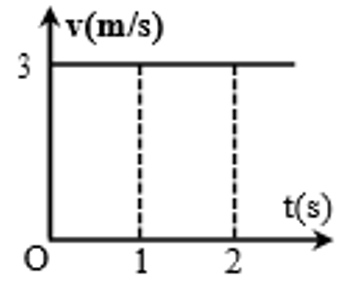
\includegraphics[scale=0.4]{figs/G10Y25B6-14}}
	\choice
	{$\SI{1}{\meter}$}
	{$\SI{2}{\meter}$}
	{\True $\SI{3}{\meter}$}
	{$\SI{4}{\meter}$}
	\loigiai{
		$$s=\left(\SI{3}{\meter/\second}\right)\cdot\left(\SI{1}{\second}\right)=\SI{3}{\meter}.$$
	}
\end{ex}

\begin{ex}\immini{Đồ thị vận tốc – thời gian của một vật chuyển động thẳng ở hình dưới. Quãng đường vật đã đi được sau $\SI{30}{\second}$ là}{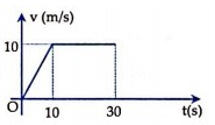
\includegraphics[scale=0.5]{figs/G10Y25B6-15}}
	\choice
	{$\SI{200}{\meter}$}
	{\True $\SI{250}{\meter}$}
	{$\SI{300}{\meter}$}
	{$\SI{350}{\meter}$}
	\loigiai{
		$$s=\dfrac{1}{2}\cdot\left(\SI{10}{\meter/\second}\right)\cdot\left(\SI{10}{\second}\right)+\left(\SI{10}{\meter/\second}\right)\cdot\left(\SI{20}{\second}\right)=\SI{250}{\meter}.$$
	}
\end{ex}

\begin{ex}
	Đồ thị vận tốc - thời gian của một vật chuyển động được biểu diễn như hình vẽ. Gọi $a_1$, $a_2$, $a_3$ lần lượt là gia tốc của vật trong các giai đoạn tương ứng là từ $t = 0$ đến $t_1 = \SI{20}{\second}$; từ $t_1 =\SI{20}{\second}$ đến $t_2 =\SI{60}{\second}$; từ $t_2 = \SI{60}{\second}$ đến $t_3 = \SI{80}{\second}$. Giá trị của $a_1, a_2, a_3$ lần lượt là
	\begin{center}
		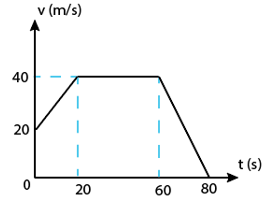
\includegraphics[scale=0.5]{figs/G10Y25B6-16}
	\end{center}
	\choice
	{$\SI{-1}{\meter/\second^2}$; $\SI{0}{\meter/\second^2}$; $\SI{2}{\meter/\second^2}$}
	{\True $\SI{1}{\meter/\second^2}$; $\SI{0}{\meter/\second^2}$; $\SI{-2}{\meter/\second^2}$}
	{$\SI{-1}{\meter/\second^2}$; $\SI{2}{\meter/\second^2}$; $\SI{0}{\meter/\second^2}$}
	{$\SI{1}{\meter/\second^2}$; $\SI{0}{\meter/\second^2}$; $\SI{2}{\meter/\second^2}$}
	\loigiai{
		\begin{align*}
			a_1&=\dfrac{\left(\SI{40}{\meter/\second}\right)-\left(\SI{20}{\meter/\second}\right)}{\SI{20}{\second}}=\SI{1}{\meter/\second^2}\\
			a_2&=\SI{0}{\meter/\second^2}\\
			a_3&=\dfrac{0-\left(\SI{40}{\meter/\second}\right)}{\SI{20}{\second}}=\SI{-2}{\meter/\second^2}
		\end{align*}
	}
\end{ex}


\begin{ex}
	\immini{	Hình bên là đồ thị vận tốc - thời gian của hai vật chuyển động thẳng cùng hướng, xuất phát từ cùng một vị trí, gốc thời gian là lúc hai vật bắt đầu chuyển động. Nhận xét sai là}{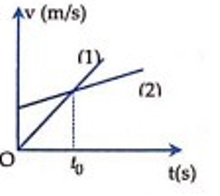
\includegraphics[scale=0.5]{figs/G10Y25B6-17}}
	\choice
	{Hai vật cùng chuyển động nhanh dần}
	{Vật 1 bắt đầu chuyển động từ trạng thái nghỉ}
	{\True Vật 2 chuyển động với gia tốc lớn hơn vật 1}
	{Ở thời điểm $t_0$, vật 1 ở phía sau vật 2}
	\loigiai{
		Độ dốc đường số 1 lớn hơn độ dốc đường 2 nên $a_1>a_2$.
	}
\end{ex}

\begin{ex}\immini{Đồ thị vận tốc - thời gian của một vật chuyển động như hình bên. Tỉ số về độ lớn gia tốc của vật trong thời gian $OA$ và $AB$ là}{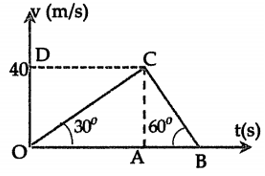
\includegraphics[scale=0.5]{figs/G10Y25B6-18}}
	\choice
	{$\dfrac{1}{2}$}
	{$1$}
	{\True $\dfrac{1}{3}$}
	{$3$}
	\loigiai{
		$$\left|\dfrac{a_1}{a_2}\right|=\left|\dfrac{\tan\SI{30}{\degree}}{\tan\SI{120}{\degree}}\right|=\dfrac{1}{3}.$$
	}
\end{ex}
\begin{ex}
	Chuyển động thẳng chậm dần đều có
	\choice
	{quỹ đạo là đường cong bất kì}
	{\True độ lớn vectơ gia tốc là một hằng số, ngược chiều với vectơ vận tốc của vật}
	{quãng đường đi được của vật không phụ thuộc vào thời gian}
	{vectơ vận tốc vuông góc với quỹ đạo của chuyển động}
	\loigiai{}
\end{ex}

\begin{ex}
	Chọn phát biểu đúng.
	\choice
	{Gia tốc của chuyển động thẳng nhanh dần đều bao giờ cũng lớn hơn gia tốc của chuyển động thẳng chậm dần đều}
	{Chuyển động thẳng nhanh dần đều có gia tốc lớn thì có vận tốc lớn}
	{Chuyển động thẳng biến đổi đều có gia tốc tăng, giảm đều theo thời gian}
	{\True Gia tốc trong chuyển động thẳng nhanh dần đều có phương, chiều và độ lớn không đổi}
	\loigiai{}
\end{ex}

\begin{ex}
	Gọi $v_0$ là vận tốc ban đầu của chuyển động. Công thức liên hệ giữa vận tốc $v$, gia tốc $a$ và quãng đường $s$ vật đi được trong chuyển động thẳng biến đổi đều là
	\choice
	{$v+v_0=\sqrt{2as}$}
	{$v-v_0=\sqrt{2as}$}
	{$v^2+v^2_0=2as$}
	{\True $v^2-v^2_0=2as$}
	\loigiai{}
\end{ex}

\begin{ex}
	Công thức tính quãng đường đi được của chuyển động thẳng nhanh dần đều là
	\choice
	{\True $s=v_0t+\dfrac{1}{2}at^2$ ($a$ và $v_0$ cùng dấu)}
	{$s=v_0t+\dfrac{1}{2}at^2$ ($a$ và $v_0$ trái dấu)}
	{$x=x_0+v_0t+\dfrac{1}{2}at^2$ ($a$ và $v_0$ cùng dấu)}
	{$x=x_0+v_0t+\dfrac{1}{2}at^2$ ($a$ và $v_0$ trái dấu)}
	\loigiai{}
\end{ex}

\begin{ex}
	Trong công thức tính vận tốc của chuyển động thẳng nhanh dần đều $v = v_0 + at$, thì
	\choice
	{$v$ luôn dương}
	{$a$ luôn dương}
	{\True tích $a\cdot v$ luôn dương}
	{tích $a\cdot v$ luôn âm}
	\loigiai{}
\end{ex}



\begin{ex}\immini{	Một vật chuyển động thẳng biến đổi đều mà vận tốc được biểu diễn bởi đồ thị như hình vẽ.\\
		Gia tốc của chuyển động là}{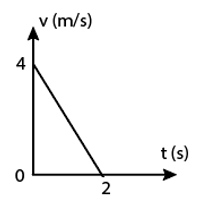
\includegraphics[scale=0.6]{figs/G10Y25B6-27}}
	\choice
	{\True $\SI{-2}{\meter/\second^2}$}
	{$\SI{2}{\meter/\second^2}$}
	{$\SI{4}{\meter/\second^2}$}
	{$\SI{-4}{\meter/\second^2}$}
	\loigiai{
		Gia tốc của chuyển động:
		$$a=\dfrac{\SI{0}{\meter/\second}-\SI{4}{\meter/\second}}{\SI{2}{\second}}=\SI{-2}{\meter/\second^2}.$$
	}
\end{ex}

\begin{ex}\immini{Một vật chuyển động thẳng biến đổi đều mà vận tốc được biểu diễn bởi đồ thị như hình vẽ.\\
		Quãng đường mà vật đi được trong $\SI{2}{\second}$ là}{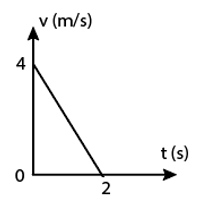
\includegraphics[scale=0.6]{figs/G10Y25B6-27}}
	\choice
	{$\SI{1}{\meter}$}
	{\True $\SI{4}{\meter}$}
	{$\SI{6}{\meter}$}
	{$\SI{8}{\meter}$}
	\loigiai{
		Quãng đường mà vật đi được trong $\SI{2}{\second}$:
		$$s=\dfrac{1}{2}\cdot\left(\SI{4}{\meter/\second}\right)\cdot\left(\SI{2}{\second}\right)=\SI{4}{\meter}.$$
	}
\end{ex}

\begin{ex}
	Một ô tô chuyển động thẳng biến đổi đều từ trạng thái nghỉ, đạt vận tốc $\SI{20}{\meter/\second}$ sau $\SI{5}{\second}$. Quãng đường mà ô tô đã đi được là
	\choice
	{$\SI{100}{\meter}$}
	{\True $\SI{50}{\meter}$}
	{$\SI{25}{\meter}$}
	{$\SI{200}{\meter}$}
	\loigiai{
		Quãng đường ô tô chuyển động:
		$$s=\dfrac{1}{2}\cdot\left(\SI{20}{\meter/\second}\right)\cdot\left(\SI{5}{\second}\right)=\SI{50}{\meter}.$$
	}
\end{ex}

\begin{ex}
	Xe ô tô đang chuyển động thẳng với tốc độ $\SI{20}{\meter/\second}$ thì bị hãm phanh chuyển động chậm dần đều. Quãng đường xe đi được từ lúc hãm phanh đến khi xe dừng hẳn là $\SI{100}{\meter}$. Gia tốc của xe là
	\choice
	{$\SI{1}{\meter/\second^2}$}
	{$\SI{-1}{\meter/\second^2}$}
	{\True $\SI{-2}{\meter/\second^2}$}
	{$\SI{5}{\meter/\second^2}$}
	\loigiai{
		Gia tốc của xe:
		$$a=\dfrac{v^2-v^2_0}{2s}=\dfrac{(\SI{0}{\meter/\second})^2-(\SI{20}{\meter/\second})^2}{2\cdot\SI{100}{\meter}}=\SI{-2}{\meter/\second^2}.$$
	}
\end{ex}

\begin{ex}
	Một ô tô chuyển động chậm dần đều. Sau $\SI{10}{\second}$ vận tốc của ô tô giảm từ $\SI{6}{\meter/\second}$ về $\SI{4}{\meter/\second}$. Quãng đường ô tô đi được trong khoảng thời gian $\SI{10}{\second}$ đó là
	\choice
	{$\SI{70}{\meter}$}
	{\True $\SI{50}{\meter}$}
	{$\SI{40}{\meter}$}
	{$\SI{100}{\meter}$}
	\loigiai{
		Quãng đường ô tô đi được trong khoảng thời gian $\SI{10}{\second}$ đó:
		$$s=\dfrac{1}{2}\cdot\left(\SI{6}{\meter/\second}+\SI{4}{\meter/\second}\right)\cdot\left(\SI{10}{\second}\right)=\SI{50}{\meter}.$$
	}
\end{ex}

\begin{ex}
	Một ô tô đang chuyển động với vận tốc $\SI{10}{\meter/\second}$ thì bắt đầu tăng ga (tăng tốc), chuyển động nhanh dần đều. Sau $\SI{20}{\second}$ ô tô đạt được vận tốc $\SI{14}{\meter/\second}$. Sau $\SI{50}{\second}$ kể từ lúc tăng tốc, gia tốc và vận tốc của ô tô lần lượt là
	\choice
	{$a=\SI{0.2}{\meter/\second^2}$ và $\SI{18}{\meter/\second}$}
	{\True $a=\SI{0.2}{\meter/\second^2}$ và $\SI{20}{\meter/\second}$}
	{$a=\SI{0.4}{\meter/\second^2}$ và $\SI{38}{\meter/\second}$}
	{$a=\SI{0.1}{\meter/\second^2}$ và $\SI{28}{\meter/\second}$}
	\loigiai{
		Gia tốc của ô tô:
		$$a=\dfrac{v-v_0}{t_1}=\dfrac{\SI{14}{\meter/\second}-\SI{10}{\meter/\second}}{\SI{20}{\second}}=\SI{0.2}{\meter/\second^2}.$$
		Vận tốc của ô tô sau $\SI{50}{\second}$:
		$$v=v_0+at=\left(\SI{10}{\meter/\second}\right)+\left(\SI{0.2}{\meter/\second^2}\right)\cdot\left(\SI{50}{\second}\right)=\SI{20}{\meter/\second}.$$
	}
\end{ex}

\begin{ex}
	Tàu hỏa đang chuyển động với vận tốc $\SI{60}{\kilo\meter/\hour}$ thì bị hãm phanh chuyển động chậm dần đều. Sau khi đi thêm được $\SI{450}{\meter}$ thì vận tốc của tàu chỉ còn $\SI{15}{\kilo\meter/\hour}$. Quãng đường tàu còn đi thêm được đến khi dừng hẳn là
	\choice
	{$\SI{60}{\meter}$}
	{$\SI{45}{\meter}$}
	{$\SI{15}{\meter}$}
	{\True $\SI{30}{\meter}$}
	\loigiai{
		Đổi đơn vị: $v_0 = \SI{60}{\kilo\meter/\hour} = \SI{16.67}{\meter/\second}$, $v = \SI{15}{\kilo\meter/\hour} = \SI{4.17}{\meter/\second}$.
		Gia tốc của tàu trong giai đoạn giảm tốc độ:
		$$a=\dfrac{v^2-v_0^2}{2s} = \dfrac{(\SI{4.17}{\meter/\second})^2 - (\SI{16.67}{\meter/\second})^2}{2 \cdot \SI{450}{\meter}} \approx \SI{-0.289}{\meter/\second^2}.$$
		Tổng quãng đường tàu đi được từ lúc hãm phanh đến khi dừng hẳn:
		$$s_{total}=\dfrac{\SI{0}{\meter/\second}^2-v_0^2}{2a} = \dfrac{-(\SI{16.67}{\meter/\second})^2}{2 \cdot (\SI{-0.289}{\meter/\second^2})} \approx \SI{480}{\meter}.$$
		Quãng đường tàu còn đi thêm được đến khi dừng hẳn là:
		$$\Delta s=s_{total}-s=\SI{480}{\meter}-\SI{450}{\meter}=\SI{30}{\meter}.$$
	}
\end{ex}

\begin{ex}\immini{Đồ thị vận tốc - thời gian của một tàu hỏa đang chuyển động thẳng có dạng như hình bên. Thời điểm $t = 0$ là lúc tàu đi qua sân ga. Vận tốc của tàu sau khi rời sân ga được $\SI{80}{\meter}$ là}{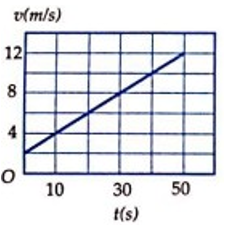
\includegraphics[scale=0.5]{figs/G10Y25B6-28}}
	\choice
	{$\SI{4}{\meter/\second}$}
	{\True $\SI{6}{\meter/\second}$}
	{$\SI{8}{\meter/\second}$}
	{$\SI{10}{\meter/\second}$}
	\loigiai{
		Gia tốc của tàu (sử dụng điểm $(\SI{0}{\second}, \SI{2}{\meter/\second})$ và $(\SI{50}{\second}, \SI{12}{\meter/\second})$ từ đồ thị):
		$$a=\dfrac{\SI{12}{\meter/\second}-\SI{2}{\meter/\second}}{\SI{50}{\second}-\SI{0}{\second}}=\dfrac{\SI{10}{\meter/\second}}{\SI{50}{\second}}=\SI{0.2}{\meter/\second^2}.$$
		Vận tốc của tàu sau khi rời ga được $\SI{80}{\meter}$ (sử dụng công thức $v^2-v_0^2=2as$, với $v_0=\SI{2}{\meter/\second}$):
		$$v=\sqrt{v^2_0+2as}=\sqrt{(\SI{2}{\meter/\second})^2+2\cdot\SI{0.2}{\meter/\second^2}\cdot\SI{80}{\meter}}=\sqrt{\SI{4}{\meter^2/\second^2}+\SI{32}{\meter^2/\second^2}}=\sqrt{\SI{36}{\meter^2/\second^2}}=\SI{6}{\meter/\second}.$$
	}
\end{ex}

\begin{ex}\immini{Một vật chuyển động thẳng biến đổi đều có đồ thị vận tốc $v$ theo thời gian $t$ như hình vẽ. Phương trình vận tốc của vật là}{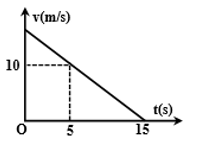
\includegraphics[scale=0.5]{figs/G10Y25B6-29}}
	\choice
	{\True $v=15-t \left(\si{\meter/\second}\right)$}
	{$v=15+t \left(\si{\meter/\second}\right)$}
	{$v=10-5t \left(\si{\meter/\second}\right)$}
	{$v=10-5t \left(\si{\meter/\second}\right)$}
	\loigiai{
		Từ đồ thị, ta thấy vận tốc ban đầu của vật là $v_0 = \SI{15}{\meter/\second}$ (tại $t=\SI{0}{\second}$).
		Gia tốc của vật:
		$$a=\dfrac{\SI{0}{\meter/\second}-\SI{15}{\meter/\second}}{\SI{15}{\second}-\SI{0}{\second}}=\SI{-1}{\meter/\second^2}.$$
		Phương trình vận tốc của vật có dạng $v=v_0+at$. Thay giá trị vào:
		$$v=\SI{15}{\meter/\second}+\left(-\SI{1}{\meter/\second^2}\right)\cdot t = 15-t \left(\si{\meter/\second}\right).$$
	}
\end{ex}

\begin{ex}\immini{	Một vật chuyển động có đồ thị vận tốc - thời gian như hình vẽ. Quãng đường đi được trong giai đoạn chuyển động thẳng chậm dần đều là}{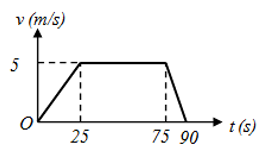
\includegraphics[scale=0.5]{figs/G10Y25B6-30}}
	\choice
	{$\SI{62.5}{\meter}$}
	{$\SI{75}{\meter}$}
	{\True $\SI{37.5}{\meter}$}
	{$\SI{100}{\meter}$}
	\loigiai{
		Giai đoạn chuyển động thẳng chậm dần đều là giai đoạn vận tốc giảm đều về 0. Trên đồ thị, đó là đoạn từ $t=\SI{0}{\second}$ đến $t=\SI{15}{\second}$, với vận tốc ban đầu là $\SI{5}{\meter/\second}$ và vận tốc cuối là $\SI{0}{\meter/\second}$.
		Quãng đường vật đi được trong giai đoạn chuyển động thẳng chậm dần đều chính là diện tích hình tam giác dưới đồ thị $v-t$ trong khoảng thời gian này:
		$$s=\dfrac{1}{2}\cdot\text{đáy}\cdot\text{chiều cao}=\dfrac{1}{2}\cdot\SI{15}{\second}\cdot\SI{5}{\meter/\second}=\SI{37.5}{\meter}.$$
	}
\end{ex}

\begin{ex}
	Một xe chuyển động nhanh dần đều với vận tốc đầu $\SI{18}{\kilo\meter/\hour}$. Trong giây thứ 5 xe đi được $\SI{14}{\meter}$. \\
	Gia tốc của xe là
	\choice
	{$\SI{4}{\meter/\second^2}$}
	{$\SI{3}{\meter/\second^2}$}
	{\True $\SI{2}{\meter/\second^2}$}
	{$\SI{6}{\meter/\second^2}$}
	\loigiai{
		Đổi đơn vị vận tốc ban đầu: $v_0 = \SI{18}{\kilo\meter/\hour} = \dfrac{18 \cdot 1000}{3600} \si{\meter/\second} = \SI{5}{\meter/\second}$.
		Công thức tính quãng đường đi được trong giây thứ $n$ là: $\Delta s_n = s(n) - s(n-1) = (v_0 n + \dfrac{1}{2} a n^2) - (v_0 (n-1) + \dfrac{1}{2} a (n-1)^2)$.
		Rút gọn công thức trên, ta được: $\Delta s_n = v_0 + a\left(n-\dfrac{1}{2}\right)$.
		Trong giây thứ 5 ($n=5$), xe đi được $\SI{14}{\meter}$:
		$$\SI{14}{\meter} = \SI{5}{\meter/\second} + a\left(\SI{5}{\second}-\dfrac{1}{2}\right) = \SI{5}{\meter/\second} + a \cdot \SI{4.5}{\second}.$$
		$$a \cdot \SI{4.5}{\second} = \SI{14}{\meter} - \SI{5}{\meter/\second} = \SI{9}{\meter}.$$
		$$a = \dfrac{\SI{9}{\meter}}{\SI{4.5}{\second}} = \SI{2}{\meter/\second^2}.$$
	}
\end{ex}

\begin{ex}
	Một xe chuyển động nhanh dần đều với vận tốc đầu $\SI{18}{\kilo\meter/\hour}$. Gia tốc của xe là $\SI{2}{\meter/\second^2}$.\\
	Quãng đường đi được trong giây thứ 10 là
	\choice
	{\True $\SI{24}{\meter}$}
	{$\SI{34}{\meter}$}
	{$\SI{14}{\meter}$}
	{$\SI{44}{\meter}$}
	\loigiai{
		Vận tốc ban đầu $v_0 = \SI{18}{\kilo\meter/\hour} = \SI{5}{\meter/\second}$.
		Gia tốc của xe $a=\SI{2}{\meter/\second^2}$.
		Công thức tính quãng đường đi được trong giây thứ $n$ là: $\Delta s_n = v_0 + a\left(n-\dfrac{1}{2}\right)$.
		Quãng đường xe đi được trong giây thứ 10 ($n=10$):
		$$\Delta s_{10} = \SI{5}{\meter/\second} + \SI{2}{\meter/\second^2}\left(\SI{10}{\second}-\dfrac{1}{2}\right) = \SI{5}{\meter/\second} + \SI{2}{\meter/\second^2}\cdot\SI{9.5}{\second} = \SI{5}{\meter/\second} + \SI{19}{\meter} = \SI{24}{\meter}.$$
	}
\end{ex}
\begin{ex}
	Một vật chuyển động thẳng chậm dần đều với tốc độ ban đầu $\SI{3}{\meter/\second}$ và gia tốc có độ lớn $\SI{2}{\meter/\second^2}$. Biết thời điểm ban đầu vật ở gốc tọa độ và chuyển động ngược chiều dương của trục tọa độ. Phương trình chuyển động của vật là
	\choice
	{$x=-3t-t^2$ (m, s)}
	{$x=3t+t^2$ (m, s)}
	{$x=-3t-t^2$ (m, s)}
	{\True $x=-3t+t^2$ (m, s)}
	\loigiai{
		Chọn gốc thời gian là khi vật bắt đầu chuyển động.
		
		Vì vật chuyển động chậm dần đều ngược chiều dương nên:
		$$
		\begin{cases}
			a\cdot v < 0 \\
			v < 0
		\end{cases}
		\Rightarrow
		\begin{cases}
			a > 0 \\
			v < 0.
		\end{cases}
		$$
		
		Kết hợp với các dữ kiện của đề bài, ta suy ra:
		$$
		\begin{cases}
			a=\SI{2}{\meter/\second^2} \\
			v_0=\SI{-3}{\meter/\second}.
		\end{cases}
		$$
		
		Phương trình chuyển động của vật có dạng:
		$x=x_0+v_0t+\dfrac{1}{2}at^2$.
		Với $x_0 = \SI{0}{\meter}$, $v_0 = \SI{-3}{\meter/\second}$, $a = \SI{2}{\meter/\second^2}$.
		Vậy, $x=-3t+\dfrac{1}{2}(2)t^2 = -3t+t^2$ (m, s).
	}
\end{ex}

\begin{ex}
	Phương trình nào sau đây là phương trình tọa độ của một vật chuyển động thẳng chậm dần đều dọc theo trục $Ox$?
	\choice
	{$s=2t-3t^2$}
	{\True $x=5t^2-2t+5$}
	{$v=4-t$}
	{$x=2-5t-t^2$}
	\loigiai{
		Phương trình chuyển động thẳng biến đổi đều có dạng tổng quát là $x = x_0 + v_0 t + \dfrac{1}{2}at^2$.
		Để chuyển động là chậm dần đều, tích $a \cdot v_0$ phải nhỏ hơn 0.
		
		Xét các phương án:
		\begin{itemize}
			\item A: $s=2t-3t^2$. Đây là phương trình quãng đường, không phải tọa độ. Ngoài ra, nếu đây là quãng đường, gia tốc $a=-6$, vận tốc ban đầu $v_0=2$. Tích $a \cdot v_0 = -12 < 0$. Nhưng đây là phương trình quãng đường, không phải phương trình tọa độ.
			\item B: $x=5t^2-2t+5$. So sánh với $x = x_0 + v_0 t + \dfrac{1}{2}at^2$, ta có:
			$x_0 = \SI{5}{\meter}$.
			$v_0 = \SI{-2}{\meter/\second}$.
			$\dfrac{1}{2}a = 5 \Rightarrow a = \SI{10}{\meter/\second^2}$.
			Tích $a \cdot v_0 = \SI{10}{\meter/\second^2} \cdot (\SI{-2}{\meter/\second}) = \SI{-20}{\meter^2/\second^3} < 0$.
			Vậy đây là chuyển động chậm dần đều.
			\item C: $v=4-t$. Đây là phương trình vận tốc, không phải tọa độ. Từ phương trình vận tốc, ta có $v_0=\SI{4}{\meter/\second}$, $a=\SI{-1}{\meter/\second^2}$. Tích $a \cdot v_0 = -4 < 0$, đây là chuyển động chậm dần đều nhưng không phải phương trình tọa độ.
			\item D: $x=2-5t-t^2$. So sánh với $x = x_0 + v_0 t + \dfrac{1}{2}at^2$, ta có:
			$x_0 = \SI{2}{\meter}$.
			$v_0 = \SI{-5}{\meter/\second}$.
			$\dfrac{1}{2}a = -1 \Rightarrow a = \SI{-2}{\meter/\second^2}$.
			Tích $a \cdot v_0 = (\SI{-2}{\meter/\second^2}) \cdot (\SI{-5}{\meter/\second}) = \SI{10}{\meter^2/\second^3} > 0$.
			Vậy đây là chuyển động nhanh dần đều.
		\end{itemize}
		Do đó, phương trình ở đáp án B là phương trình tọa độ của một vật chuyển động thẳng chậm dần đều.
	}
\end{ex}

\begin{ex}
	Một vật chuyển động thẳng chậm dần đều với tốc độ ban đầu $\SI{4}{\meter/\second}$ và gia tốc có độ lớn $\SI{2}{\meter/\second^2}$. Biết thời điểm ban đầu vật ở gốc tọa độ và chuyển động cùng chiều dương của trục tọa độ. Phương trình chuyển động của vật là
	\choice
	{$x=-4t-t^2$ (m, s)}
	{\True $x=4t-t^2$ (m, s)}
	{$x=4t-t^2$ (m, s)}
	{$x=-4t+t^2$ (m, s)}
	\loigiai{
		Chọn gốc thời gian là khi vật bắt đầu chuyển động.
		
		Vì vật chuyển động chậm dần đều cùng chiều dương nên:
		$$
		\begin{cases}
			a\cdot v <0 \\
			v > 0
		\end{cases}
		\Rightarrow
		\begin{cases}
			a < 0 \\
			v > 0.
		\end{cases}
		$$
		
		Kết hợp với các dữ kiện của đề bài, ta suy ra:
		$$
		\begin{cases}
			a=\SI{-2}{\meter/\second^2} \\
			v_0=\SI{4}{\meter/\second}.
		\end{cases}
		$$
		
		Phương trình chuyển động của vật có dạng:
		$x=x_0+v_0t+\dfrac{1}{2}at^2$.
		Với $x_0 = \SI{0}{\meter}$, $v_0 = \SI{4}{\meter/\second}$, $a = \SI{-2}{\meter/\second^2}$.
		Vậy, $x=4t+\dfrac{1}{2}(-2)t^2 = 4t-t^2$ (m, s).
	}
\end{ex}

\begin{ex}
	Phương trình toạ độ của một vật chuyển động thẳng biến đổi đều là: $x = 20t^2 + 40t + 6$ (cm; s). Tính gia tốc và tính chất của chuyển động.
	\choice
	{\True $\SI{40}{\centi\meter/\second^2}$; vật chuyển động nhanh dần đều}
	{$\SI{40}{\centi\meter/\second^2}$; vật chuyển động chậm dần đều}
	{$\SI{20}{\centi\meter/\second^2}$; vật chuyển động nhanh dần đều}
	{$\SI{20}{\centi\meter/\second^2}$; vật chuyển động chậm dần đều}
	\loigiai{
		Phương trình tọa độ tổng quát của chuyển động thẳng biến đổi đều là $x = x_0 + v_0t + \dfrac{1}{2}at^2$.
		So sánh với phương trình đã cho $x = 6 + 40t + 20t^2$, ta có:
		$v_0 = \SI{40}{\centi\meter/\second}$.
		$\dfrac{1}{2}a = 20 \Rightarrow a = \SI{40}{\centi\meter/\second^2}$.
		
		Để xác định tính chất chuyển động, ta xét tích $a \cdot v_0$:
		$a \cdot v_0 = \SI{40}{\centi\meter/\second^2} \cdot \SI{40}{\centi\meter/\second} = \SI{1600}{\centi\meter^2/\second^3}$.
		Vì $a \cdot v_0 > 0$ nên vật chuyển động thẳng **nhanh dần đều**.
	}
\end{ex}

\begin{ex}
	Cùng một lúc, vật thứ nhất đi từ A hướng đến B với vận tốc ban đầu $\SI{10}{\meter/\second}$, chuyển động chậm dần đều với gia tốc $\SI{0.2}{\meter/\second^2}$; vật thứ hai chuyển động nhanh dần đều, không vận tốc đầu từ B về A với gia tốc $\SI{0.4}{\meter/\second^2}$. Biết $AB = \SI{560}{\meter}$. Chọn A làm gốc tọa độ, chiều dương hướng từ A đến B, gốc thời gian là lúc hai vật bắt đầu chuyển động. Phương trình chuyển động của hai vật là
	\choice
	{\True $x_1=10t-0,1t^2$ $\left(\si{\meter}\right)$; $x_2=560-0,2t^2$ $\left(\si{\meter}\right)$}
	{$x_1=10t-0,2t^2$ $\left(\si{\meter}\right)$; $x_2=560-0,4t^2$ $\left(\si{\meter}\right)$}
	{$x_1=10t+0,1t^2$ $\left(\si{\meter}\right)$; $x_2=560+0,2t^2$ $\left(\si{\meter}\right)$}
	{$x_1=10t+0,2t^2$ $\left(\si{\meter}\right)$; $x_2=560+0,4t^2$ $\left(\si{\meter}\right)$}
	\loigiai{
		Chọn gốc tọa độ tại A, chiều dương từ A đến B, gốc thời gian là lúc hai vật bắt đầu chuyển động.
		
		**Đối với vật thứ nhất (đi từ A đến B):**
		Vận tốc ban đầu $v_{01} = \SI{10}{\meter/\second}$.
		Chuyển động chậm dần đều, cùng chiều dương nên gia tốc $a_1$ phải âm. Độ lớn gia tốc là $\SI{0.2}{\meter/\second^2}$, vậy $a_1 = -\SI{0.2}{\meter/\second^2}$.
		Phương trình chuyển động: $x_1 = x_{01} + v_{01}t + \dfrac{1}{2}a_1t^2$.
		Với $x_{01} = \SI{0}{\meter}$.
		$x_1 = \SI{0}{\meter} + \SI{10}{\meter/\second} \cdot t + \dfrac{1}{2}(\SI{-0.2}{\meter/\second^2})t^2 = 10t - 0.1t^2$ (m).
		
		**Đối với vật thứ hai (đi từ B về A):**
		Vận tốc ban đầu $v_{02} = \SI{0}{\meter/\second}$ (không vận tốc đầu).
		Vị trí ban đầu $x_{02} = AB = \SI{560}{\meter}$.
		Chuyển động nhanh dần đều về A (ngược chiều dương) nên gia tốc $a_2$ phải âm. Độ lớn gia tốc là $\SI{0.4}{\meter/\second^2}$, vậy $a_2 = -\SI{0.4}{\meter/\second^2}$.
		Phương trình chuyển động: $x_2 = x_{02} + v_{02}t + \dfrac{1}{2}a_2t^2$.
		$x_2 = \SI{560}{\meter} + \SI{0}{\meter/\second} \cdot t + \dfrac{1}{2}(\SI{-0.4}{\meter/\second^2})t^2 = 560 - 0.2t^2$ (m).
		
		Vậy, phương trình chuyển động của hai vật là:
		$x_1=10t-0,1t^2$ $\left(\si{\meter}\right)$
		$x_2=560-0,2t^2$ $\left(\si{\meter}\right)$.
	}
\end{ex}

\begin{ex}
	Cùng một lúc ở hai điểm cách nhau $\SI{300}{\meter}$, có hai ô tô đi ngược chiều nhau. Xe thứ nhất đi từ A có tốc độ ban đầu là $\SI{10}{\meter/\second}$, xe thứ hai đi từ B với tốc độ ban đầu là $\SI{20}{\meter/\second}$. Biết xe đi từ A chuyển động nhanh dần đều, xe đi từ B chuyển động chậm dần đều và hai xe chuyển động với gia tốc có cùng độ lớn $\SI{2}{\meter/\second^2}$.
	a. Khoảng cách giữa hai xe sau $\SI{5}{\second}$ là
	\choice
	{$\SI{100}{\meter}$}
	{\True $\SI{150}{\meter}$}
	{$\SI{200}{\meter}$}
	{$\SI{400}{\meter}$}
	\loigiai{
		Chọn A làm gốc tọa độ, chiều dương từ A đến B, gốc thời gian là lúc hai xe bắt đầu chuyển động.
		
		**Đối với xe thứ nhất (đi từ A):**
		$x_{01} = \SI{0}{\meter}$.
		$v_{01} = \SI{10}{\meter/\second}$.
		Xe đi từ A chuyển động nhanh dần đều, cùng chiều dương nên $a_1 = \SI{2}{\meter/\second^2}$.
		Phương trình chuyển động của xe 1: $x_1 = \SI{0}{\meter} + \SI{10}{\meter/\second} \cdot t + \dfrac{1}{2}(\SI{2}{\meter/\second^2})t^2 = 10t + t^2$ (m).
		
		**Đối với xe thứ hai (đi từ B):**
		$x_{02} = \SI{300}{\meter}$.
		$v_{02} = \SI{-20}{\meter/\second}$ (do đi ngược chiều dương).
		Xe đi từ B chuyển động chậm dần đều, ngược chiều dương ($v_{02} < 0$) nên gia tốc $a_2$ phải dương để $a_2 \cdot v_{02} < 0$. Vậy $a_2 = \SI{2}{\meter/\second^2}$.
		Phương trình chuyển động của xe 2: $x_2 = \SI{300}{\meter} + (\SI{-20}{\meter/\second}) \cdot t + \dfrac{1}{2}(\SI{2}{\meter/\second^2})t^2 = 300 - 20t + t^2$ (m).
		
		**a. Khoảng cách giữa hai xe sau $\SI{5}{\second}$:**
		Tại $t=\SI{5}{\second}$:
		$x_1(\SI{5}{\second}) = 10 \cdot \SI{5}{\second} + (\SI{5}{\second})^2 = \SI{50}{\meter} + \SI{25}{\meter} = \SI{75}{\meter}$.
		$x_2(\SI{5}{\second}) = \SI{300}{\meter} - 20 \cdot \SI{5}{\second} + (\SI{5}{\second})^2 = \SI{300}{\meter} - \SI{100}{\meter} + \SI{25}{\meter} = \SI{225}{\meter}$.
		Khoảng cách giữa hai xe: $\Delta x = |x_2 - x_1| = |\SI{225}{\meter} - \SI{75}{\meter}| = \SI{150}{\meter}$.
	}
\end{ex}

\begin{ex}
	Lúc $\SI{7}{\hour}$, hai ô tô bắt đầu khởi hành từ hai điểm A, B cách nhau $\SI{2400}{\meter}$, chuyển động nhanh dần đều và ngược chiều nhau. Ô tô đi từ A có gia tốc $\SI{1}{\meter / \second \squared}$, còn ô tô đi từ B có gia tốc $\SI{2}{\meter / \second \squared}$. Chọn chiều dương hướng từ A đến B, gốc thời gian lúc $\SI{7}{\hour}$. Xác định vị trí hai xe gặp nhau.
	\choice
	{$\SI{1600}{\meter}$}
	{$\SI{1200}{\meter}$}
	{\True $\SI{800}{\meter}$}
	{$\SI{2400}{\meter}$}
	\loigiai{
		Chọn chiều dương hướng từ A đến B, gốc tọa độ tại A, gốc thời gian lúc $\SI{7}{\hour}$.
		
		**Đối với ô tô đi từ A:**
		$x_{0A} = \SI{0}{\meter}$.
		$v_{0A} = \SI{0}{\meter/\second}$ (do bắt đầu khởi hành từ trạng thái đứng yên).
		$a_A = \SI{1}{\meter/\second^2}$.
		Phương trình chuyển động của xe A: $x_A = x_{0A} + v_{0A}t + \dfrac{1}{2}a_At^2 = \SI{0}{\meter} + \SI{0}{\meter/\second} \cdot t + \dfrac{1}{2}(\SI{1}{\meter/\second^2})t^2 = 0.5t^2$ (m).
		
		**Đối với ô tô đi từ B:**
		$x_{0B} = \SI{2400}{\meter}$.
		$v_{0B} = \SI{0}{\meter/\second}$ (bắt đầu khởi hành).
		Chuyển động ngược chiều dương, nên gia tốc $a_B = -\SI{2}{\meter/\second^2}$.
		Phương trình chuyển động của xe B: $x_B = x_{0B} + v_{0B}t + \dfrac{1}{2}a_Bt^2 = \SI{2400}{\meter} + \SI{0}{\meter/\second} \cdot t + \dfrac{1}{2}(\SI{-2}{\meter/\second^2})t^2 = 2400 - t^2$ (m).
		
		**Hai xe gặp nhau:** $x_A = x_B$.
		$0.5t^2 = 2400 - t^2$.
		$1.5t^2 = 2400$.
		$t^2 = \dfrac{2400}{1.5} = 1600$.
		$t = \sqrt{1600} = \SI{40}{\second}$ (thời gian phải dương).
		
		**Vị trí gặp nhau:** Thay $t=\SI{40}{\second}$ vào phương trình $x_A$ (hoặc $x_B)$.
		$x_A = 0.5 \cdot (\SI{40}{\second})^2 = 0.5 \cdot 1600 = \SI{800}{\meter}$.
		(Kiểm tra lại $x_B = 2400 - (\SI{40}{\second})^2 = 2400 - 1600 = \SI{800}{\meter}$.).
		Vậy, hai xe gặp nhau tại vị trí cách A $\SI{800}{\meter}$.
	}
\end{ex}

\begin{ex}
	Lúc $\SI{1}{\hour}$, một xe qua A với tốc độ $\SI{10}{\meter/\second}$, chuyển động nhanh dần đều với gia tốc $\SI{1}{\meter/\second^2}$ đuổi theo một xe đạp đang chuyển động nhanh dần đều qua B với tốc độ đầu là $\SI{2}{\meter/\second}$ và với gia tốc là $\SI{0.5}{\meter/\second^2}$. Sau $\SI{20}{\second}$ thì xe đuổi kịp xe đạp. Tính khoảng cách AB.
	\choice
	{$\SI{300}{\meter}$}
	{$\SI{250}{\meter}$}
	{$\SI{200}{\meter}$}
	{\True $\SI{260}{\meter}$}
	\loigiai{
		Chọn gốc tọa độ tại A, chiều dương hướng từ A đến B, gốc thời gian là lúc $\SI{1}{\hour}$ (lúc xe ô tô qua A).
		
		**Đối với xe ô tô (từ A):**
		$x_{0C} = \SI{0}{\meter}$.
		$v_{0C} = \SI{10}{\meter/\second}$.
		$a_C = \SI{1}{\meter/\second^2}$.
		Phương trình chuyển động của xe ô tô: $x_C = \SI{0}{\meter} + \SI{10}{\meter/\second} \cdot t + \dfrac{1}{2}(\SI{1}{\meter/\second^2})t^2 = 10t + 0.5t^2$ (m).
		
		**Đối với xe đạp (từ B):**
		Gọi khoảng cách AB là $L$. Vậy $x_{0X} = L$.
		$v_{0X} = \SI{2}{\meter/\second}$.
		$a_X = \SI{0.5}{\meter/\second^2}$.
		Phương trình chuyển động của xe đạp: $x_X = L + \SI{2}{\meter/\second} \cdot t + \dfrac{1}{2}(\SI{0.5}{\meter/\second^2})t^2 = L + 2t + 0.25t^2$ (m).
		
		Hai xe gặp nhau sau $\SI{20}{\second}$, tức là tại $t=\SI{20}{\second}$, $x_C = x_X$.
		Thay $t=\SI{20}{\second}$ vào các phương trình:
		$x_C(\SI{20}{\second}) = 10 \cdot \SI{20}{\second} + 0.5 \cdot (\SI{20}{\second})^2 = \SI{200}{\meter} + 0.5 \cdot \SI{400}{\meter^2/\second^2} = \SI{200}{\meter} + \SI{200}{\meter} = \SI{400}{\meter}$.
		$x_X(\SI{20}{\second}) = L + 2 \cdot \SI{20}{\second} + 0.25 \cdot (\SI{20}{\second})^2 = L + \SI{40}{\meter} + 0.25 \cdot \SI{400}{\meter^2/\second^2} = L + \SI{40}{\meter} + \SI{100}{\meter} = L + \SI{140}{\meter}$.
		
		Khi gặp nhau: $x_C = x_X$.
		$\SI{400}{\meter} = L + \SI{140}{\meter}$.
		$L = \SI{400}{\meter} - \SI{140}{\meter} = \SI{260}{\meter}$.
		Vậy, khoảng cách AB là $\SI{260}{\meter}$.
	}
\end{ex}

\begin{ex}
	Vật (1) xuất phát lúc 7h30 từ A chuyển động thẳng nhanh dần đều với tốc độ ban đầu $\SI{2}{\meter/\second}$, gia tốc $\SI{1}{\meter/\second^2}$ hướng về B. Sau 2 giây, vật (2) xuất phát từ B chuyển động thẳng nhanh dần đều không vận tốc đầu về A với gia tốc $\SI{2}{\meter/\second^2}$. Khoảng cách $AB = \SI{134}{\meter}$.\\
	a. Tìm thời gian và vị trí hai vật gặp nhau.
	\choice
	{$t=\SI{5}{\second}$, $x_1=\SI{70}{\meter}$}
	{$t=\SI{10}{\second}$, $x_1=\SI{50}{\meter}$}
	{\True $t=\SI{10}{\second}$, $x_1=\SI{70}{\meter}$}
	{$t=\SI{5}{\second}$, $x_1=\SI{50}{\meter}$}
	\loigiai{
		Chọn gốc tọa độ tại A, chiều dương hướng từ A đến B.
		Chọn gốc thời gian là lúc vật (1) xuất phát ($\SI{7}{\hour}\SI{30}{\minute}$).
		
		**Phương trình chuyển động của vật (1) (từ A):**
		$x_{01} = \SI{0}{\meter}$.
		$v_{01} = \SI{2}{\meter/\second}$.
		$a_1 = \SI{1}{\meter/\second^2}$.
		$x_1(t) = \SI{0}{\meter} + \SI{2}{\meter/\second} \cdot t + \dfrac{1}{2}(\SI{1}{\meter/\second^2})t^2 = 2t + 0.5t^2$ (m).
		
		**Phương trình chuyển động của vật (2) (từ B về A):**
		Vật (2) xuất phát sau 2 giây, tức là tại thời điểm $t' = t - \SI{2}{\second}$ (với $t$ là thời gian tính từ lúc vật 1 xuất phát).
		$x_{02} = AB = \SI{134}{\meter}$.
		$v_{02} = \SI{0}{\meter/\second}$ (không vận tốc đầu).
		Chuyển động về A (ngược chiều dương) nên gia tốc $a_2 = -\SI{2}{\meter/\second^2}$.
		$x_2(t) = \SI{134}{\meter} + \SI{0}{\meter/\second} \cdot (t-\SI{2}{\second}) + \dfrac{1}{2}(\SI{-2}{\meter/\second^2})(t-\SI{2}{\second})^2 = 134 - (t-\SI{2}{\second})^2$ (m).
		
		**Khi hai vật gặp nhau:** $x_1(t) = x_2(t)$.
		$2t + 0.5t^2 = 134 - (t-\SI{2}{\second})^2$.
		$2t + 0.5t^2 = 134 - (t^2 - 4t + 4)$.
		$2t + 0.5t^2 = 134 - t^2 + 4t - 4$.
		$2t + 0.5t^2 = 130 + 4t - t^2$.
		$1.5t^2 - 2t - 130 = 0$.
		
		Giải phương trình bậc hai $1.5t^2 - 2t - 130 = 0$:
		$\Delta = (-2)^2 - 4(1.5)(-130) = 4 + 780 = 784$.
		$\sqrt{\Delta} = \sqrt{784} = 28$.
		
		$t = \dfrac{-(-2) \pm 28}{2 \cdot 1.5} = \dfrac{2 \pm 28}{3}$.
		$t_1 = \dfrac{2+28}{3} = \dfrac{30}{3} = \SI{10}{\second}$.
		$t_2 = \dfrac{2-28}{3} = -\dfrac{26}{3}$ (loại vì thời gian phải dương).
		
		Vậy hai vật gặp nhau sau $\SI{10}{\second}$ kể từ lúc vật (1) xuất phát.
		
		Vị trí gặp nhau: Thay $t=\SI{10}{\second}$ vào phương trình $x_1(t)$.
		$x_1(\SI{10}{\second}) = 2 \cdot \SI{10}{\second} + 0.5 \cdot (\SI{10}{\second})^2 = \SI{20}{\meter} + 0.5 \cdot \SI{100}{\meter} = \SI{20}{\meter} + \SI{50}{\meter} = \SI{70}{\meter}$.
		Vị trí gặp nhau cách A $\SI{70}{\meter}$.
	}
\end{ex}
\begin{ex}
	Vật (1) xuất phát lúc 7h30 từ A chuyển động thẳng nhanh dần đều với tốc độ ban đầu $\SI{2}{\meter/\second}$, gia tốc $\SI{1}{\meter/\second^2}$ hướng về B. Sau 2 giây, vật (2) xuất phát từ B chuyển động thẳng nhanh dần đều không vận tốc đầu về A với gia tốc $\SI{2}{\meter/\second^2}$. Khoảng cách $AB = \SI{134}{\meter}$.\\
	b. Sau bao lâu kể từ lúc bắt đầu chuyển động 2 vật cách nhau $\SI{50}{\meter}$?
	\choice
	{$\SI{15}{\second}$ và $\SI{11.6}{\second}$}
	{$\SI{8}{\second}$ và $\SI{16}{\second}$}
	{$\SI{15}{\second}$ và $\SI{16}{\second}$}
	{\True $\SI{8}{\second}$ và $\SI{11.6}{\second}$}
	\loigiai{
		Tiếp tục từ phần a.
		
		**b. Sau bao lâu kể từ lúc bắt đầu chuyển động 2 vật cách nhau $\SI{50}{\meter}$?**
		Khoảng cách giữa hai vật là $\Delta x = |x_1(t) - x_2(t)|$. Ta cần tìm $t$ sao cho $|x_1(t) - x_2(t)| = \SI{50}{\meter}$.
		Ta có $x_1(t) = 2t + 0.5t^2$ và $x_2(t) = 134 - (t-2)^2$.
		$x_1(t) - x_2(t) = (2t + 0.5t^2) - (134 - (t-2)^2)$
		$x_1(t) - x_2(t) = 2t + 0.5t^2 - 134 + (t^2 - 4t + 4)$
		$x_1(t) - x_2(t) = 2t + 0.5t^2 - 134 + t^2 - 4t + 4$
		$x_1(t) - x_2(t) = 1.5t^2 - 2t - 130$.
		
		Ta có hai trường hợp:
		**Trường hợp 1:** $x_1(t) - x_2(t) = \SI{50}{\meter}$.
		$1.5t^2 - 2t - 130 = 50$.
		$1.5t^2 - 2t - 180 = 0$.
		Giải phương trình bậc hai:
		$\Delta = (-2)^2 - 4(1.5)(-180) = 4 + 1080 = 1084$.
		$\sqrt{\Delta} = \sqrt{1084} \approx 32.92$.
		
		$t = \dfrac{2 \pm 32.92}{3}$.
		$t_1 = \dfrac{2+32.92}{3} = \dfrac{34.92}{3} \approx \SI{11.64}{\second}$.
		$t_2 = \dfrac{2-32.92}{3} = -\dfrac{30.92}{3}$ (loại).
		
		**Trường hợp 2:** $x_1(t) - x_2(t) = -\SI{50}{\meter}$.
		$1.5t^2 - 2t - 130 = -50$.
		$1.5t^2 - 2t - 80 = 0$.
		Giải phương trình bậc hai:
		$\Delta = (-2)^2 - 4(1.5)(-80) = 4 + 480 = 484$.
		$\sqrt{\Delta} = \sqrt{484} = 22$.
		
		$t = \dfrac{2 \pm 22}{3}$.
		$t_1 = \dfrac{2+22}{3} = \dfrac{24}{3} = \SI{8}{\second}$.
		$t_2 = \dfrac{2-22}{3} = -\dfrac{20}{3}$ (loại).
		
		Vậy có hai thời điểm mà hai vật cách nhau $\SI{50}{\meter}$ là $\SI{8}{\second}$ và khoảng $\SI{11.6}{\second}$.
	}
\end{ex}
\Closesolutionfile{ans}
\subsection{TRẮC NGHIỆM ĐÚNG SAI}
\setcounter{ex}{0}
\Opensolutionfile{ans}[ans/G10Y25B6-TF]

\Closesolutionfile{ans}
\subsection{TRẢ LỜI NGẮN}
\setcounter{ex}{0}
\Opensolutionfile{ans}[ans/G10Y25B6-SA]

\Closesolutionfile{ans}
\subsection{TỰ LUẬN}
\setcounter{ex}{0}
\Opensolutionfile{ans}[ans/G10Y25B6-TL]
\begin{ex}
	Một chiếc ô tô đang chạy với vận tốc $\SI{23}{\meter/\second}$ thì chạy chầm dần. Sau $\SI{10}{\second}$, vận tốc của ô tô chỉ còn $\SI{11}{\meter/\second}$. Tính gia tốc của ô tô.
	\loigiai{
		Gia tốc của ô tô:
		$$a=\dfrac{v-v_0}{\Delta t}=\dfrac{\SI{11}{\meter/\second}-\SI{23}{\meter/\second}}{\SI{10}{\second}}=\SI{-1.2}{\meter/\second^2}.$$
	}
\end{ex}

\begin{ex}
	Một con báo đang chạy với vận tốc $\SI{30}{\meter/\second}$ thì chuyển động chậm dần khi tới gần một con suối. Trong 3 giây, vận tốc của nó giảm còn $\SI{9}{\meter/\second}$. Tính gia tốc của con báo.
	\loigiai{
		Gia tốc của con báo là:
		$$a = \dfrac{v_2 - v_1}{\Delta t} = \dfrac{\SI{9}{\meter/\second}-\SI{30}{\meter/\second}}{\SI{3}{\second}} = -\SI{7}{\meter/\second^2}.$$
	}
\end{ex}

\begin{ex}
	Một ô tô tăng tốc từ trạng thái đứng yên, sau $\SI{6}{s}$ ô tô đạt vận tốc $\SI{18}{\meter/\second}$. Tính độ lớn gia tốc trung bình của ô tô trong khoảng thời gian trên.
	\loigiai{
		Gia tốc của ô tô:
		$$a = \dfrac{v_2 - v_1}{t} = \dfrac{\SI{18}{\meter/\second} - \SI{0}{\meter/\second}}{\SI{6}{\second}} = \SI{3}{\meter/\second^2}.$$
	}
\end{ex}

\begin{ex}
	Bảng dưới đây ghi vận tốc tức thời đo bởi tốc kế của một ô tô sau các khoảng thời gian $\SI{2}{s}$ kể từ khi bắt đầu chạy trên một đường thẳng.
	
	\begin{center}
		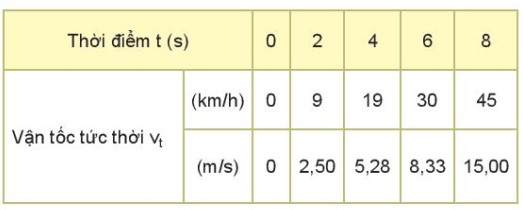
\includegraphics[scale=1]{figs/G10Y25B6-19}
	\end{center}
	
	\begin{enumerate}[label=\alph*)]
		\item Xác định độ biến thiên vận tốc sau $\SI{8}{s}$ của chuyển động trên.
		\item Xác định độ biến thiên của vận tốc sau mỗi giây của chuyển động trên trong $\SI{4}{s}$ đầu và trong $\SI{4}{s}$ cuối.
	\end{enumerate}
	\loigiai{
		\begin{enumerate}[label=\alph*)]
			\item 
			Độ biến thiên vận tốc sau 8 giây là
			$$\Delta v = v_8 - v_0 = \SI{45}{\kilo\meter/\hour}.$$
			\item Độ biến thiên vận tốc trong 4 giây đầu là
			$$\Delta v = v_4 - v_0 = \SI{5.28}{\meter/\second}.$$
			
			Độ biến thiên của vận tốc sau mỗi giây của chuyển động trên trong 4 giây đầu là :
			$$\dfrac{\Delta v}{\Delta t} = \dfrac{\SI{5.28}{\meter/\second}}{\SI{4}{\second}} = \SI{1.32}{\meter/\second^2}.$$
			
			Độ biến thiên vận tốc trong 4 giây cuối là: 
			$$\Delta v' = v_8 - v_4 = \SI{9.72}{\meter/\second}.$$
			
			Độ biến thiên của vận tốc sau mỗi giây của chuyển động trên trong 4 giây cuối là:
			$$\dfrac{\Delta v'}{\Delta t} = \dfrac{\SI{9.72}{\meter/\second}}{\SI{4}{\second}} = \SI{2.43}{\meter/\second^2}.$$ 
		\end{enumerate}
	}
\end{ex}

\begin{ex}
	Đồ thị mô tả sự thay đổi vận tốc theo thời gian trong chuyển động của một ô tô thể thao đang chạy thử về phía Bắc. Tính gia tốc của ô tô:
	\begin{center}
		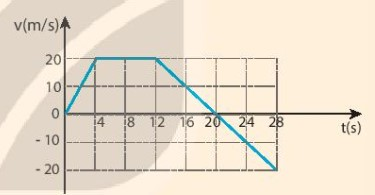
\includegraphics[scale=1]{figs/G10Y25B6-20}
	\end{center}
	
	\begin{enumerate}[label=\alph*)]
		\item Trong $\SI{4}{s}$ đầu tiên.
		\item Từ giây thứ 4 đến giây thứ 12.
		\item Từ giây thứ 12 đến giây thứ 20.
		\item Từ giây thứ 20 đến giây thứ 28.
	\end{enumerate}
	\loigiai{
		\begin{enumerate}[label=\alph*)]
			\item Trong $\SI{4}{s}$
			$$a_1 = \dfrac{\SI{20}{\meter/\second} -\SI{0}{\meter/\second}}{\SI{4}{\second}- \SI{0}{\second}} = \SI{5}{\meter/\second^2}.$$
			
			\item Từ giây thứ 4 đến giây thứ 12
			$$a_2 = \dfrac{\SI{20}{\meter/\second} - \SI{20}{\meter/\second}}{\SI{12}{\second}-\SI{4}{\second}} = \SI{0}{\meter/\second^2}.$$
			
			\item Từ giây thứ 12 đến giây thứ 20
			$$a_3 = \dfrac{\SI{0}{\meter/\second} - \SI{20}{\meter/\second}}{\SI{20}{\second}-\SI{12}{\second}} = -\SI{2.5}{\meter/\second^2}.$$
			
			\item Từ giây thứ 20 đến giây thứ 28
			$$a_4 = \dfrac{\SI{-20}{\meter/\second} - \SI{0}{\meter/\second}}{\SI{28}{\second} -\SI{20}{\second}} = -\SI{2.5}{\meter/\second^2}.$$
		\end{enumerate}
	}
\end{ex}

\begin{ex}
	Một quả bóng tennis đang ba với tốc độ $\SI{25}{\meter/\second}$ theo hướng đông thì chạm vào tường chắn và bay trở lại với tốc độ $\SI{15}{\meter/\second}$ theo hướng tây. Thời gian va chạm giữa bóng và tường là $\SI{0.05}{\second}$.
	\begin{enumerate}[label=\alph*)]
		\item Tính sự thay đổi tốc độ của quả bóng.
		\item Tính sự thay đổi vận tốc của quả bóng.
		\item Tính gia tốc của quả bóng trong thời gian tiếp xúc với tường.
	\end{enumerate}
	\loigiai{
		\begin{enumerate}[label=\alph*)]
			\item $\Delta\left|v\right|=\left|\left|\vec{v_2}\right|-\left|\vec{v_1}\right|\right|=\left|\SI{15}{\meter/\second}-\SI{25}{\meter/\second}\right|=\SI{10}{\meter/\second}$.
			\item Chọn chiều dương là chiều từ tây sang đông 
			$\Rightarrow\begin{cases}
				v_1=\SI{-25}{\meter/\second}\\
				v_2=\SI{15}{\meter/\second}
			\end{cases}$.\\
			Độ biến thiên vận tốc của quả bóng
			$$\Delta v=v_2-v_1=\SI{15}{\meter/\second}-(\SI{-25}{\meter/\second})=\SI{40}{\meter/\second}.$$
			\item Gia tốc của quả bóng trong thời gian tiếp xúc với tường:
			$$a=\dfrac{\Delta v}{\Delta t}=\dfrac{\SI{40}{\meter/\second}}{\SI{0.05}{\second}}=\SI{800}{\meter/\second^2}.$$
		\end{enumerate}
	}
\end{ex}

\begin{ex}
	Trên hình \ref{fig:TP008-P-12}, a), b) và c) là đồ thị vận tốc - thời gian $\left(v-t\right)$ của các vật chuyển động thẳng theo một hướng xác định. Các đồ thị gia tốc theo thời gian của các chuyển động này $\left(a-t\right)$, được biểu diễn theo thứ tự xáo trộn là d), e) và g). Hãy chọn từng cặp đồ thị $v-t$ và đồ thị $a-t$ ứng với mỗi chuyển động.
	\begin{center}
		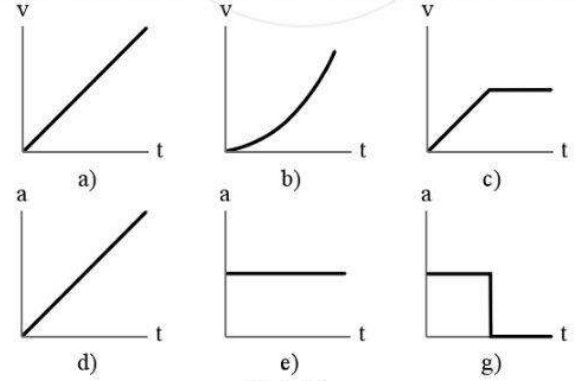
\includegraphics[scale=0.5]{figs/G10Y25B6-21}
		\captionof{figure}{}
		\label{fig:TP008-P-12}
	\end{center}
	\loigiai{
		Đồ thị a) có hệ số góc không đổi, cho biết gia tốc không đổi; gia tốc tương ứng của đồ thị a) là đồ thị e).\\
		Đồ thị b) biểu diễn một tốc độ tăng liên tục nhưng độ dốc của đồ thị tăng dần theo thời gian. Do đó, gia tốc tương ứng của đồ thị b) được biểu diễn phù hợp nhất là đồ thị d).\\
		Đồ thị c) mô tả 2 giai đoạn. Ban đầu, vận tốc tăng đều theo thời gian (độ dốc của đồ thị không đổi), do đó gia tốc của vật là hằng số. Sau đó, vận tốc của vật không đổi, do đó gia tốc của vật bằng 0. Đồ thị phù hợp nhất cho gia tốc của vật ở hình c) là đồ thị hình g).
	}
\end{ex}

\begin{ex}
	Đồ thị vận tốc - thời gian của một vật chuyển động dọc theo trục $x$ được thể hiện trong hình \ref{fig: TP008-P-11}. Xác định gia tốc trung bình của vật trong các khoảng thời gian
	\begin{center}
		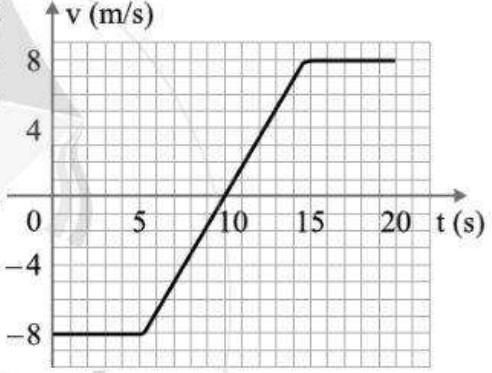
\includegraphics[scale=0.5]{figs/G10Y25B6-22}
		\captionof{figure}{}
		\label{fig: TP008-P-11}
	\end{center}
	\begin{enumerate}[label=\alph*)]
		\item $t=\SI{5.00}{\second}$ đến $t=\SI{15.0}{\second}$.
		\item $t=\SI{0}{\second}$ đến $t=\SI{20.0}{\second}$.
	\end{enumerate}
	\loigiai{
		\begin{enumerate}[label=\alph*)]
			\item Gia tốc trung bình của vật trong khoảng thời gian từ $t=\SI{5.00}{\second}$ đến $t=\SI{15.0}{\second}$:
			$$a_1=\dfrac{v_{t=\SI{15}{\second}}-v_{t=\SI{5}{\second}}}{\Delta t}=\dfrac{\left(\SI{8}{\meter/\second}\right)-\left(\SI{-8}{\meter/\second}\right)}{\SI{15}{\second}-\SI{5}{\second}}=\SI{1.6}{\meter/\second^2}.$$
			\item Gia tốc trung bình của vật trong khoảng thời gian từ $t=\SI{0}{\second}$ đến $t=\SI{20.0}{\second}$:
			$$a_2=\dfrac{v_{t=\SI{20}{\second}}-v_{t=\SI{0}{\second}}}{\Delta t}=\dfrac{\left(\SI{8}{\meter/\second}\right)-\left(\SI{-8}{\meter/\second}\right)}{\SI{20}{\second}-\SI{0}{\second}}=\SI{0.8}{\meter/\second^2}.$$
		\end{enumerate}
	}
\end{ex}

\begin{ex}
	Một tài xế xe tải đang chuyển động đều với tốc độ cho phép trên đường cao tốc trong khoảng thời gian $\Delta t$. Khi nhìn thấy biển báo "Đoạn đường hay xảy ra tai nạn", tài xế quyết định giảm tốc độ. Sau khoảng thời gian $\Delta t_1$, tài xế quan sát thấy một tai nạn đột ngột xảy ra ở phía trước. Do đó tài xế hãm phanh gấp để dừng lại trong khoảng thời gian ngắn $\Delta t_2$ để tránh va chạm. Giả sử trong suốt quá trình chuyển động, xe tải luôn chạy trên đường thẳng.
	\begin{enumerate}[label=\alph*)]
		\item Vẽ đồ thị vận tốc - thời gian biểu diễn quá trình chuyển động của xe tải.
		\item Độ dốc của đồ thị trong trường hợp nào lớn nhất?
	\end{enumerate}
	\loigiai{
		\begin{enumerate}[label=\alph*)]
			\item Đồ thị biểu diễn quá trình chuyển động của xe tải
			\begin{center}
				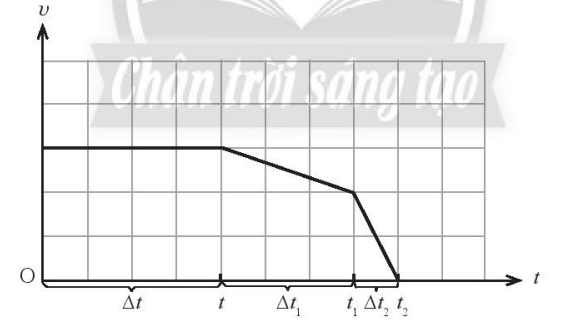
\includegraphics[scale=0.5]{figs/G10Y25B6-23}
			\end{center}
			\item Trong thời gian $\Delta t_2$ độ dốc của đồ thị vận tốc - thời gian là lớn nhất.
		\end{enumerate}
	}
\end{ex}

\begin{ex}
	Một vật chuyển động có đồ thị $(v-t)$ như hình bên.
	\begin{center}
		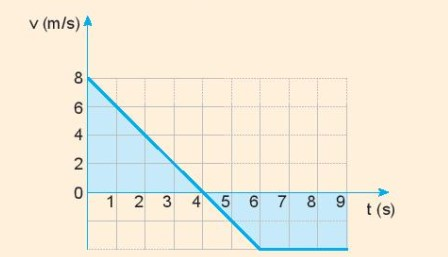
\includegraphics[scale=1]{figs/G10Y25B6-24}
	\end{center}
	\begin{enumerate}[label=\alph*)]
		\item Mô tả chuyển động của vật.
		\item Tính độ dịch chuyển trong 4 giây đầu, 2 giây tiếp theo và 3 giây cuối.
		\item Tính gia tốc của chuyển động trong 4 giây đầu.
		\item Tính gia tốc của chuyển động từ giây thứ 4 đến giây thứ 6.
	\end{enumerate}
	\loigiai{
		\begin{enumerate}[label=\alph*)]
			\item 
			\begin{itemize}
				\item Trong 4 giây đầu tiên: chuyển động chậm dần đều từ $\SI{8}{\meter/\second}$ đến $\SI{0}{\meter/\second}$.
				\item Từ giây thứ 4 đến giây thứ 6: vật chuyển động nhanh dần đều theo chiều âm với vận tốc từ $\SI{0}{\meter/\second}$ đến $-\SI{2}{\meter/\second}$.
				\item Từ giây thứ 6 đến giây thứ 9: chuyển động thẳng đều với vận tốc $-\SI{2}{\meter/\second}$.
			\end{itemize}
			\item 
			\begin{itemize}
				\item Trong 4 giây đầu:
				Độ dịch chuyển bằng diện tích tam giác vuông có cạnh đáy là $t$ và chiều cao là $v$.
				$$d_1 = \dfrac{1}{2} \cdot \SI{8}{\meter/\second} \cdot \SI{4}{\second} = \SI{16}{\meter}.$$
				\item Trong 2 giây tiếp theo (từ giây thứ 4 đến giây thứ 6):
				Độ dịch chuyển bằng diện tích tam giác vuông có cạnh đáy là $t$ và chiều cao là $v$.
				$$d_2 = \dfrac{1}{2} \cdot \left(-\SI{2}{\meter/\second}\right) \cdot \SI{2}{\second} = -\SI{2}{\meter}.$$
				\item Trong 3 giây cuối (từ giây thứ 6 đến giây thứ 9):
				Độ dịch chuyển bằng diện tích hình chữ nhật có chiều dài là $t$ và chiều rộng là $v$.
				$$d_3 = \left(-\SI{2}{\meter/\second}\right) \cdot \SI{3}{\second} = -\SI{6}{\meter}.$$
			\end{itemize}
			\item Gia tốc của chuyển động trong 4 giây đầu:
			$$a = \dfrac{v_f - v_i}{\Delta t} =\dfrac{\SI{0}{\meter/\second} - \SI{8}{\meter/\second}}{\SI{4}{\second}-\SI{0}{\second}}= -\SI{2}{\meter/\second^2}.$$
			\item Gia tốc của chuyển động từ giây thứ 4 đến giây thứ 6:
			$$a = \dfrac{v_f - v_i}{\Delta t} =\dfrac{-\SI{2}{\meter/\second} - \SI{0}{\meter/\second}}{\SI{6}{\second}-\SI{4}{\second}}= -\SI{1}{\meter/\second^2}.$$
		\end{enumerate}
	}
\end{ex}

\begin{ex}
	Chuyển động của một vật có đồ thị vận tốc theo thời gian như hình vẽ. Tổng quãng đường vật đã đi bằng bao nhiêu?
	\begin{center}
		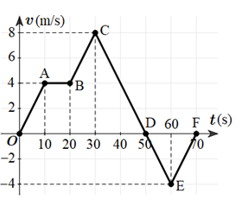
\includegraphics[scale=0.5]{figs/G10Y25B6-25}
	\end{center}
	\loigiai{
		Tổng quãng đường vật đi được là tổng diện tích tuyệt đối dưới đồ thị $v-t$:
		$$s = \left(\dfrac{1}{2}\cdot\SI{4}{\meter/\second}\cdot\SI{10}{\second}\right) + \left(\SI{4}{\meter/\second}\cdot\SI{10}{\second}\right) + \left(\dfrac{1}{2}\cdot\left(\SI{4}{\meter/\second}+\SI{8}{\meter/\second}\right)\cdot\SI{10}{\second}\right) + \left(\dfrac{1}{2}\cdot\SI{8}{\meter/\second}\cdot\SI{20}{\second}\right) + \left(\dfrac{1}{2}\cdot\SI{8}{\meter/\second}\cdot\SI{10}{\second}\right) + \left(\dfrac{1}{2}\cdot\SI{4}{\meter/\second}\cdot\SI{10}{\second}\right) = \SI{260}{\meter}.$$
	}
\end{ex}

\begin{ex}
	Một quả bóng bàn được bắn ra theo phương ngang với vận tốc ban đầu bằng không đến va chạm vào tường và bật lại trong khoảng thời gian rất ngắn. Hình bên là đồ thị $\left(v-t\right)$ mô tả chuyển động của quả bóng trong $\SI{20}{\second}$ đầu tiên. Tính quãng đường mà quả bóng bay được sau $\SI{20}{\second}$ kể từ lúc bắt đầu chuyển động.
	\begin{center}
		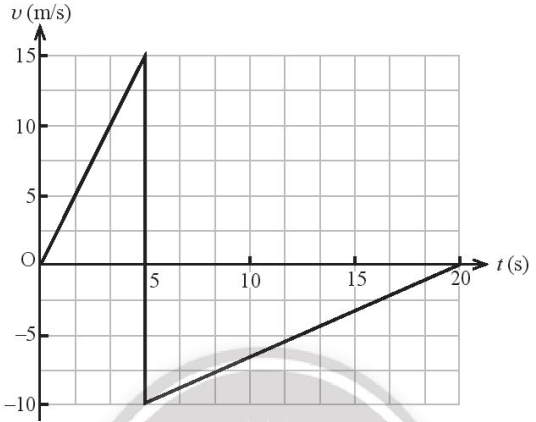
\includegraphics[scale=0.5]{figs/G10Y25B6-26}
	\end{center}
	\loigiai{
		Quãng đường bóng bay được là tổng diện tích tuyệt đối dưới đồ thị $v-t$:
		$$s = \left(\dfrac{1}{2}\cdot\SI{15}{\meter/\second}\cdot\SI{15}{\second}\right) + \left(\dfrac{1}{2}\cdot\SI{10}{\meter/\second}\cdot\left(\SI{20}{\second}-\SI{15}{\second}\right)\right) = \SI{112.5}{\meter} + \SI{25}{\meter} = \SI{137.5}{\meter}.$$
	}
\end{ex}
\begin{ex}
	Từ các đồ thị trong hình:
	\begin{center}
		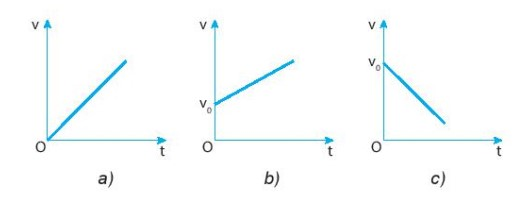
\includegraphics[scale=1]{figs/G10Y25B6-31}
	\end{center}
	
	\begin{enumerate}[label=\alph*)]
		\item Hãy viết công thức về mối liên hệ giữa $v$ với $a$ và $t$ của từng chuyển động ứng với từng đồ thị trong hình.
		\item Chuyển động nào là chuyển động nhanh dần đều, chậm dần đều?
	\end{enumerate}
	\loigiai{
		\begin{enumerate}[label=\alph*)]
			\item 
			- Đồ thị a (đường thẳng đi qua gốc tọa độ, $v$ tỉ lệ thuận với $t$): $$v=at.$$
			
			- Đồ thị b (đường thẳng không đi qua gốc tọa độ, $v$ tăng theo $t$): $$v = v_0 + at.$$
			
			- Đồ thị c (đường thẳng không đi qua gốc tọa độ, $v$ giảm theo $t$): $$v = v_0 -at.$$
			\item 
			
			- Chuyển động nhanh dần đều là: đồ thị a (xuất phát từ nghỉ và $v$ tăng) và b (vận tốc ban đầu dương, gia tốc dương).
			
			- Chuyển động chậm dần đều: đồ thị c (vận tốc ban đầu dương, gia tốc âm, $v$ giảm về 0).
		\end{enumerate}
	}
\end{ex}

\begin{ex}
	Trong một cuộc thi chạy, một vận động viên chạy nhanh dần đều từ trạng thái đứng yên với gia tốc $\SI{5}{\meter/\second^2}$ trong $\SI{2}{\second}$ đầu tiên. Tính tốc độ của vận động viên sau $\SI{2}{\second}$.
	\loigiai{
		Tốc độ của vận động viên sau $\SI{2}{\second}$ đầu tiên:
		Vì vận động viên chạy từ trạng thái đứng yên nên vận tốc ban đầu $v_0 = \SI{0}{\meter/\second}$.
		Sử dụng công thức vận tốc: $v = v_0 + at$.
		$$v = \SI{0}{\meter/\second} + \SI{5}{\meter/\second^2} \cdot \SI{2}{\second} = \SI{10}{\meter/\second}.$$
	}
\end{ex}

\begin{ex}
	Một xe máy đang chuyển động thẳng với vận tốc $\SI{10}{\meter/\second}$ thì tăng tốc. Sau $\SI{5}{\second}$ đạt vận tốc $\SI{12}{\meter/\second}.$
	
	\begin{enumerate}[label=\alph*)]
		\item Tính gia tốc của xe.
		\item Nếu sau khi đạt vận tốc $\SI{12}{\meter/\second}$, xe chuyển động chậm dần với gia tốc có độ lớn bằng gia tốc trên thì sau bao lâu xe dừng lại?
	\end{enumerate}
	\loigiai{
		\begin{enumerate}[label=\alph*)]
			\item Gia tốc của xe:
			$$a = \dfrac{\Delta v}{\Delta t} = \dfrac{\SI{12}{\meter/\second} - \SI{10}{\meter/\second}}{\SI{5}{\second}} = \dfrac{\SI{2}{\meter/\second}}{\SI{5}{\second}} = \SI{0.4}{\meter/\second^2}.$$
			
			\item Thời gian xe dừng lại:
			Xe chuyển động chậm dần với gia tốc có độ lớn bằng gia tốc trên, tức là gia tốc lúc này là $a' = -\SI{0.4}{\meter/\second^2}$.
			Vận tốc ban đầu cho giai đoạn này là $v_0' = \SI{12}{\meter/\second}$ và vận tốc cuối khi xe dừng lại là $v = \SI{0}{\meter/\second}\Rightarrow t = \SI{30}{\second}.$
		\end{enumerate}
	}
\end{ex}

\begin{ex}
	Một ô tô đang chuyển động thẳng đều với vận tốc $\SI{45}{\kilo\meter/\hour}$ bỗng tăng ga chuyển động nhanh dần đều.
	\begin{enumerate}[label=\alph*)]
		\item Tính gia tốc của xe biết rằng sau $\SI{30}{\second}$ ô tô đạt vận tốc $\SI{72}{\kilo\meter/\hour}$.
		\item Trong quá trình tăng tốc nói trên, vào thời điểm nào kể từ lúc tăng tốc, vận tốc của xe là $\SI{64.8}{\kilo\meter/\hour}$?
	\end{enumerate}
	\loigiai{
		Đổi đơn vị vận tốc:
		$v_0 = \SI{45}{\kilo\meter/\hour} = \dfrac{45 \cdot 1000}{3600} \si{\meter/\second} = \SI{12.5}{\meter/\second}.$
		$v = \SI{72}{\kilo\meter/\hour} = \dfrac{72 \cdot 1000}{3600} \si{\meter/\second} = \SI{20}{\meter/\second}.$
		
		Chọn chiều dương là chiều chuyển động.
		
		\begin{enumerate}[label=\alph*)]
			\item Gia tốc của xe là:
			Sử dụng công thức gia tốc: $a = \dfrac{v-v_0}{t}$.
			$$a = \dfrac{\SI{20}{\meter/\second}-\SI{12.5}{\meter/\second}}{\SI{30}{\second}}= \dfrac{\SI{7.5}{\meter/\second}}{\SI{30}{\second}} = \SI{0.25}{\meter/\second^2}.$$
			
			\item Thời điểm vận tốc của xe là $\SI{64.8}{\kilo\meter/\hour}$:
			Đổi đơn vị vận tốc: $v' = \SI{64.8}{\kilo\meter/\hour} = \dfrac{64.8 \cdot 1000}{3600} \si{\meter/\second} = \SI{18}{\meter/\second}.$
			Sử dụng công thức vận tốc: $v' = v_0 + at'$.
			$$\SI{18}{\meter/\second} = \SI{12.5}{\meter/\second} + \SI{0.25}{\meter/\second^2} \cdot t'.$$
			$$\SI{0.25}{\meter/\second^2} \cdot t' = \SI{18}{\meter/\second} - \SI{12.5}{\meter/\second} = \SI{5.5}{\meter/\second}.$$
			$$t' = \dfrac{\SI{5.5}{\meter/\second}}{\SI{0.25}{\meter/\second^2}} = \SI{22}{\second}.$$
		\end{enumerate}
	}
\end{ex}

\begin{ex}
	Một người đi xe đạp lên dốc dài $\SI{50}{\meter}$. Tốc độ ở dưới chân dốc là $\SI{18}{\kilo\meter/\hour}$ và ở đầu dốc lúc đến nơi là $\SI{3}{\meter/\second}$. Tính gia tốc của chuyển động và thời gian lên dốc. Coi chuyển động trên là chuyển động chậm dần đều.
	\loigiai{
		Đổi đơn vị vận tốc ban đầu: $v_0 = \SI{18}{\kilo\meter/\hour} = \dfrac{18 \cdot 1000}{3600} \si{\meter/\second} = \SI{5}{\meter/\second}$.
		
		Gia tốc của người đi xe đạp:
		Sử dụng công thức liên hệ giữa vận tốc, gia tốc và quãng đường: $v^2 - v_0^2 = 2as$.
		$$(\SI{3}{\meter/\second})^2 - (\SI{5}{\meter/\second})^2 = 2 \cdot a \cdot \SI{50}{\meter}.$$
		$$\SI{9}{\meter^2/\second^2} - \SI{25}{\meter^2/\second^2} = \SI{100}{\meter} \cdot a.$$
		$$-\SI{16}{\meter^2/\second^2} = \SI{100}{\meter} \cdot a.$$
		$$a = \dfrac{-\SI{16}{\meter^2/\second^2}}{\SI{100}{\meter}} = \SI{-0.16}{\meter/\second^2}.$$
		
		Thời gian lên dốc:
		Sử dụng công thức vận tốc: $v = v_0 + at$.
		$$\SI{3}{\meter/\second} = \SI{5}{\meter/\second} + (\SI{-0.16}{\meter/\second^2}) \cdot \Delta t.$$
		$$\Delta t = \dfrac{\SI{3}{\meter/\second} - \SI{5}{\meter/\second}}{-\SI{0.16}{\meter/\second^2}} = \dfrac{-\SI{2}{\meter/\second}}{-\SI{0.16}{\meter/\second^2}} = \SI{12.5}{\second}.$$
	}
\end{ex}

\begin{ex}
	Một người đạp xe trên đường thẳng với tốc độ $\SI{4}{\meter/\second}$ thì bóp thắng để giảm tốc với gia tốc có độ lớn không đổi là $\SI{0.5}{\meter/\second^2}$. Xác định thời gian và quãng đường xe đi được từ khi bóp thắng đến khi dừng lại.
	\loigiai{
		Vận tốc ban đầu của xe là $v_0 = \SI{4}{\meter/\second}$.
		Khi xe dừng lại, vận tốc cuối là $v = \SI{0}{\meter/\second}$.
		Vì xe giảm tốc, gia tốc sẽ có giá trị âm: $a = -\SI{0.5}{\meter/\second^2}$.
		
		Quãng đường xe đi được từ khi bóp thắng đến khi dừng lại:
		Sử dụng công thức liên hệ giữa vận tốc, gia tốc và quãng đường: $v^2 - v_0^2 = 2as$.
		$$(\SI{0}{\meter/\second})^2 - (\SI{4}{\meter/\second})^2 = 2 \cdot (-\SI{0.5}{\meter/\second^2}) \cdot s.$$
		$$\SI{0}{\meter^2/\second^2} - \SI{16}{\meter^2/\second^2} = -\SI{1}{\meter/\second^2} \cdot s.$$
		$$-\SI{16}{\meter^2/\second^2} = -\SI{1}{\meter/\second^2} \cdot s.$$
		$$s = \dfrac{-\SI{16}{\meter^2/\second^2}}{-\SI{1}{\meter/\second^2}} = \SI{16}{\meter}.$$
		
		Thời gian từ khi bóp thắng đến khi dừng lại:
		Sử dụng công thức vận tốc: $v = v_0 + at$.
		$$\SI{0}{\meter/\second} = \SI{4}{\meter/\second} + (-\SI{0.5}{\meter/\second^2}) \cdot \Delta t.$$
		$$-\SI{4}{\meter/\second} = -\SI{0.5}{\meter/\second^2} \cdot \Delta t.$$
		$$\Delta t = \dfrac{-\SI{4}{\meter/\second}}{-\SI{0.5}{\meter/\second^2}} = \SI{8}{\second}.$$
	}
\end{ex}

\begin{ex}
	Khi đang chạy với tốc độ $\SI{36}{\kilo\meter/\hour}$ thì ô tô bắt đầu chạy xuống dốc. Nhưng do bị mất phanh nên ô tô chuyển động thẳng nhanh dần đều với gia tốc $\SI{0.2}{\meter/\second^2}$ xuống hết dốc có độ dài $\SI{960}{\meter}$. Khoảng thời gian ô tô chạy xuống hết đoạn dốc là bao nhiêu?
	\loigiai{
		Đổi đơn vị vận tốc ban đầu: $v_0 = \SI{36}{\kilo\meter/\hour} = \dfrac{36 \cdot 1000}{3600} \si{\meter/\second} = \SI{10}{\meter/\second}.$
		Gia tốc $a=\SI{0.2}{\meter/\second^2}$.
		Quãng đường dốc $s=\SI{960}{\meter}$.
		
		Sử dụng công thức quãng đường trong chuyển động thẳng biến đổi đều: $s=v_0t+\dfrac{1}{2}at^2$.
		Thay các giá trị vào phương trình:
		$$\SI{960}{\meter}=\SI{10}{\meter/\second}\cdot t+\dfrac{1}{2}\cdot\SI{0.2}{\meter/\second^2}\cdot t^2$$
		$$\SI{960}{\meter}=\SI{10}{\meter/\second}\cdot t+\SI{0.1}{\meter/\second^2}\cdot t^2$$
		Sắp xếp lại thành phương trình bậc hai theo $t$:
		$$\SI{0.1}{\meter/\second^2} \cdot t^2 + \SI{10}{\meter/\second} \cdot t - \SI{960}{\meter} = 0$$
		Để giải phương trình bậc hai $At^2 + Bt + C = 0$, ta sử dụng công thức nghiệm $t = \dfrac{-B \pm \sqrt{B^2 - 4AC}}{2A}$.
		Trong đó $A = 0.1$, $B = 10$, $C = -960$.
		$$t = \dfrac{-10 \pm \sqrt{10^2 - 4 \cdot 0.1 \cdot (-960)}}{2 \cdot 0.1}$$
		$$t = \dfrac{-10 \pm \sqrt{100 + 384}}{0.2}$$
		$$t = \dfrac{-10 \pm \sqrt{484}}{0.2}$$
		$$t = \dfrac{-10 \pm 22}{0.2}$$
		Vì thời gian $t$ phải có giá trị dương, ta chọn nghiệm:
		$$t = \dfrac{-10 + 22}{0.2} = \dfrac{12}{0.2} = \SI{60}{\second}.$$
		Khoảng thời gian ô tô chạy xuống hết đoạn dốc là $\SI{60}{\second}$.
	}
\end{ex}

\begin{ex}
	Đồ thị vận tốc - thời gian ở hình mô tả chuyển động của một chú chó con đang chạy trong một ngõ thẳng và hẹp.
	\begin{center}
		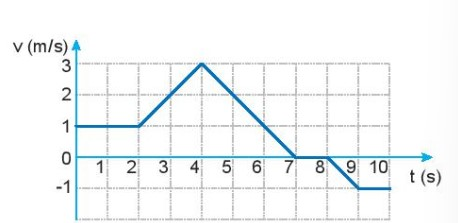
\includegraphics[scale=1]{figs/G10Y25B6-32}
	\end{center}
	
	\begin{enumerate}[label=\alph*)]
		\item Hãy mô tả chuyển động của chú chó.
		\item Tính quãng đường đi được và độ dịch chuyển của chú chó sau $\SI{2}{\second}$; $\SI{4}{\second}$; $\SI{7}{\second}$ và $\SI{10}{\second}$ bằng đồ thị.
	\end{enumerate}
	\loigiai{
		\begin{enumerate}[label=\alph*)]
			\item Mô tả chuyển động của chú chó:
			- Trong $\SI{2}{\second}$ đầu tiên (từ $t=\SI{0}{\second}$ đến $t=\SI{2}{\second}$): Chuyển động thẳng đều với vận tốc $v=\SI{1}{\meter/\second}$.
			- Từ giây thứ 2 đến giây thứ 4 (từ $t=\SI{2}{\second}$ đến $t=\SI{4}{\second}$): Chuyển động nhanh dần đều (vận tốc tăng từ $\SI{1}{\meter/\second}$ đến $\SI{3}{\meter/\second}$).
			- Từ giây thứ 4 đến giây thứ 7 (từ $t=\SI{4}{\second}$ đến $t=\SI{7}{\second}$): Chuyển động chậm dần đều (vận tốc giảm từ $\SI{3}{\meter/\second}$ về $\SI{0}{\meter/\second}$).
			- Từ giây thứ 7 đến giây thứ 8 (từ $t=\SI{7}{\second}$ đến $t=\SI{8}{\second}$): Chú chó dừng lại (vận tốc bằng $\SI{0}{\meter/\second}$).
			- Từ giây thứ 8 đến giây thứ 9 (từ $t=\SI{8}{\second}$ đến $t=\SI{9}{\second}$): Chuyển động nhanh dần đều theo chiều âm (vận tốc giảm từ $\SI{0}{\meter/\second}$ đến $\SI{-1}{\meter/\second}$).
			- Từ giây thứ 9 đến giây thứ 10 (từ $t=\SI{9}{\second}$ đến $\SI{10}{\second}$): Chuyển động thẳng đều theo chiều âm với vận tốc $v=-\SI{1}{\meter/\second}$.
			
			\item Tính quãng đường đi được và độ dịch chuyển của chú chó:
			Quãng đường đi được là tổng diện tích các phần dưới đồ thị (lấy giá trị tuyệt đối của vận tốc), còn độ dịch chuyển là tổng đại số diện tích các phần.
			
			- Sau $\SI{2}{\second}$:
			Đây là giai đoạn chuyển động thẳng đều. Quãng đường $s_1$ và độ dịch chuyển $d_1$ là diện tích hình chữ nhật từ $\SI{0}{\second}$ đến $\SI{2}{\second}$:
			$$s_1 = d_1 = \text{vận tốc} \cdot \text{thời gian} = \SI{1}{\meter/\second} \cdot \SI{2}{\second} = \SI{2}{\meter}.$$
			
			- Sau $\SI{4}{\second}$:
			Quãng đường $s_2$ và độ dịch chuyển $d_2$ là tổng quãng đường sau $\SI{2}{\second}$ và diện tích hình thang (từ $\SI{2}{\second}$ đến $\SI{4}{\second}$):
			$$s_2 = d_2 = s_1 + \dfrac{1}{2} (\text{đáy nhỏ}+\text{đáy lớn})\cdot\text{chiều cao} = \SI{2}{\meter} + \dfrac{1}{2} (\SI{1}{\meter/\second}+\SI{3}{\meter/\second})(\SI{4}{\second}-\SI{2}{\second})$$
			$$s_2 = \SI{2}{\meter} + \dfrac{1}{2} (\SI{4}{\meter/\second})(\SI{2}{\second}) = \SI{2}{\meter} + \SI{4}{\meter} = \SI{6}{\meter}.$$
			
			- Sau $\SI{7}{\second}$:
			Quãng đường $s_3$ và độ dịch chuyển $d_3$ là tổng quãng đường sau $\SI{4}{\second}$ và diện tích hình tam giác (từ $\SI{4}{\second}$ đến $\SI{7}{\second}$):
			$$s_3 = d_3 = s_2 + \dfrac{1}{2} \cdot \text{đáy} \cdot \text{chiều cao} = \SI{6}{\meter} + \dfrac{1}{2} (\SI{7}{\second}-\SI{4}{\second}) \cdot \SI{3}{\meter/\second}$$
			$$s_3 = \SI{6}{\meter} + \dfrac{1}{2} (\SI{3}{\second})(\SI{3}{\meter/\second}) = \SI{6}{\meter} + \SI{4.5}{\meter} = \SI{10.5}{\meter}.$$
			
			- Sau $\SI{10}{\second}$:
			+ Quãng đường:
			Quãng đường từ $\SI{7}{\second}$ đến $\SI{8}{\second}$ là $\SI{0}{\meter}$ (do vận tốc bằng $\SI{0}{\meter/\second}$).
			Quãng đường từ $\SI{8}{\second}$ đến $\SI{9}{\second}$ (diện tích hình tam giác dưới trục hoành):
			$$s_{8-9} = \dfrac{1}{2} \cdot (\SI{9}{\second}-\SI{8}{\second}) \cdot |\SI{-1}{\meter/\second}| = \dfrac{1}{2} \cdot \SI{1}{\second} \cdot \SI{1}{\meter/\second} = \SI{0.5}{\meter}.$$
			Quãng đường từ $\SI{9}{\second}$ đến $\SI{10}{\second}$ (diện tích hình chữ nhật dưới trục hoành):
			$$s_{9-10} = (\SI{10}{\second}-\SI{9}{\second}) \cdot |\SI{-1}{\meter/\second}| = \SI{1}{\second} \cdot \SI{1}{\meter/\second} = \SI{1}{\meter}.$$
			Tổng quãng đường:
			$$s_{total} = s_3 + s_{8-9} + s_{9-10} = \SI{10.5}{\meter} + \SI{0.5}{\meter} + \SI{1}{\meter} = \SI{12}{\meter}.$$
			
			+ Độ dịch chuyển:
			Độ dịch chuyển từ $\SI{7}{\second}$ đến $\SI{8}{\second}$ là $\SI{0}{\meter}$.
			Độ dịch chuyển từ $\SI{8}{\second}$ đến $\SI{9}{\second}$ (diện tích tam giác, có dấu âm):
			$$d_{8-9} = -\dfrac{1}{2} \cdot (\SI{9}{\second}-\SI{8}{\second}) \cdot \SI{1}{\meter/\second} = -\SI{0.5}{\meter}.$$
			Độ dịch chuyển từ $\SI{9}{\second}$ đến $\SI{10}{\second}$ (diện tích hình chữ nhật, có dấu âm):
			$$d_{9-10} = -(\SI{10}{\second}-\SI{9}{\second}) \cdot \SI{1}{\meter/\second} = -\SI{1}{\meter}.$$
			Tổng độ dịch chuyển:
			$$d_{total} = d_3 + d_{8-9} + d_{9-10} = \SI{10.5}{\meter} - \SI{0.5}{\meter} - \SI{1}{\meter} = \SI{9}{\meter}.$$
		\end{enumerate}
	}
\end{ex}

\begin{ex}
	Dựa vào đồ thị vận tốc - thời gian ở hình \ref{fig:TP009-P-4}, hãy xác định tính chất chuyển động và độ dịch chuyển trong từng giai đoạn chuyển động của xe.
	\begin{center}
		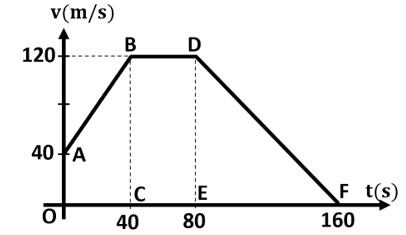
\includegraphics[scale=0.5]{figs/G10Y25B6-33}
		\captionof{figure}{}
		\label{fig:TP009-P-4}
	\end{center}
	\loigiai{
		\begin{itemize}
			\item Trong giai đoạn từ $\SI{0}{\second}$ đến $\SI{40}{\second}$ (đoạn OA trên đồ thị):
			Vận tốc tăng từ $\SI{0}{\meter/\second}$ đến $\SI{120}{\meter/\second}$.
			Tính chất chuyển động: Vật chuyển động nhanh dần đều.
			Độ dịch chuyển của vật trong giai đoạn này (diện tích hình tam giác dưới đồ thị):
			$$d_1=\dfrac{1}{2}\cdot\text{đáy}\cdot\text{chiều cao}=\dfrac{1}{2}\cdot\SI{40}{\second}\cdot\SI{120}{\meter/\second}=\SI{2400}{\meter}.$$
			
			\item Trong giai đoạn từ $\SI{40}{\second}$ đến $\SI{80}{\second}$ (đoạn AB trên đồ thị):
			Vận tốc không đổi và bằng $\SI{120}{\meter/\second}$.
			Tính chất chuyển động: Vật chuyển động thẳng đều.
			Độ dịch chuyển của vật trong giai đoạn này (diện tích hình chữ nhật dưới đồ thị):
			$$d_2=\text{chiều dài}\cdot\text{chiều rộng}=\left(\SI{80}{\second}-\SI{40}{\second}\right)\cdot\SI{120}{\meter/\second}=\SI{40}{\second}\cdot\SI{120}{\meter/\second}=\SI{4800}{\meter}.$$
			
			\item Trong giai đoạn từ $\SI{80}{\second}$ đến $\SI{160}{\second}$ (đoạn BC trên đồ thị):
			Vận tốc giảm từ $\SI{120}{\meter/\second}$ về $\SI{0}{\meter/\second}$.
			Tính chất chuyển động: Vật chuyển động chậm dần đều.
			Gia tốc trong giai đoạn này:
			$$a_3=\dfrac{v_{cuoi}-v_{dau}}{t_{cuoi}-t_{dau}}=\dfrac{\SI{0}{\meter/\second}-\SI{120}{\meter/\second}}{\SI{160}{\second}-\SI{80}{\second}}=\dfrac{-\SI{120}{\meter/\second}}{\SI{80}{\second}}=\SI{-1.5}{\meter/\second^2}.$$
			Độ dịch chuyển của vật trong giai đoạn này (diện tích hình tam giác dưới đồ thị):
			$$d_3=\dfrac{1}{2}\cdot\text{đáy}\cdot\text{chiều cao}=\dfrac{1}{2}\cdot\left(\SI{160}{\second}-\SI{80}{\second}\right)\cdot\SI{120}{\meter/\second}=\SI{4800}{\meter}.$$
		\end{itemize}
	}
\end{ex}

\begin{ex}
	Một vận động viên đua xe đạp đường dài vượt qua vạch đích với vận tốc $\SI{10}{\meter/\second}$. Sau đó vận động viên này đi chậm dần đều thêm $\SI{20}{\meter}$ mới dừng lại. Coi chuyển động của vận động viên là thẳng.
	\begin{enumerate}[label=\alph*)]
		\item Tính gia tốc của vận động viên trong đoạn đường sau khi qua vạch đích.
		\item Tính thời gian vận động viên đó cần để dừng lại kể từ khi cán đích.
		\item Tính tốc độ trung bình của người đó trên quãng đường dừng xe.
	\end{enumerate}
	\loigiai{
		Vận tốc ban đầu khi qua vạch đích là $v_0=\SI{10}{\meter/\second}$.
		Khi dừng lại, vận tốc cuối là $v=\SI{0}{\meter/\second}$.
		Quãng đường đi được thêm là $s=\SI{20}{\meter}$.
		
		\begin{enumerate}[label=\alph*)]
			\item Tính gia tốc của vận động viên trong đoạn đường sau khi qua vạch đích:
			Sử dụng công thức liên hệ giữa vận tốc, gia tốc và quãng đường: $v^2 - v_0^2 = 2as$.
			$$(\SI{0}{\meter/\second})^2 - (\SI{10}{\meter/\second})^2 = 2 \cdot a \cdot \SI{20}{\meter}.$$
			$$\SI{0}{\meter^2/\second^2} - \SI{100}{\meter^2/\second^2} = \SI{40}{\meter} \cdot a.$$
			$$-\SI{100}{\meter^2/\second^2} = \SI{40}{\meter} \cdot a.$$
			$$a = \dfrac{-\SI{100}{\meter^2/\second^2}}{\SI{40}{\meter}} = \SI{-2.5}{\meter/\second^2}.$$
			
			\item Tính thời gian vận động viên đó cần để dừng lại kể từ khi cán đích:
			Sử dụng công thức vận tốc: $v = v_0 + at$.
			$$\SI{0}{\meter/\second} = \SI{10}{\meter/\second} + (\SI{-2.5}{\meter/\second^2}) \cdot \Delta t.$$
			$$-\SI{10}{\meter/\second} = -\SI{2.5}{\meter/\second^2} \cdot \Delta t.$$
			$$\Delta t = \dfrac{-\SI{10}{\meter/\second}}{-\SI{2.5}{\meter/\second^2}} = \SI{4}{\second}.$$
			
			\item Tính tốc độ trung bình của người đó trên quãng đường dừng xe:
			Tốc độ trung bình được tính bằng tổng quãng đường chia cho tổng thời gian:
			$$v_{tb} = \dfrac{s}{\Delta t} = \dfrac{\SI{20}{\meter}}{\SI{4}{\second}} = \SI{5}{\meter/\second}.$$
		\end{enumerate}
	}
\end{ex}
\begin{ex}
	Một chất điểm chuyển động dọc theo trục $Ox$ với phương trình $x=5+10t-0,25t^2$; trong đó $x$ tính bằng mét, $t$ tính bằng giây.
	\begin{enumerate}
		\item Xác định gia tốc và vận tốc của chất điểm. Chuyển động của chất điểm là loại chuyển động nào?
		\item Tìm vận tốc tức thời của chất điểm lúc $t=\SI{4}{\second}$.
	\end{enumerate}
	\loigiai{
		Phương trình chuyển động của chất điểm có dạng tổng quát: $x = x_0 + v_0 t + \dfrac{1}{2}at^2$.
		So sánh với phương trình đã cho $x = 5 + 10t - 0.25t^2$:
		\begin{enumerate}[label=\alph*)]
			\item 
			Gia tốc: $\dfrac{1}{2}a = -0.25 \Rightarrow a = \SI{-0.5}{\meter/\second^2}$.\\
			Vận tốc ban đầu: $v_0 = \SI{10}{\meter/\second}$.
			Để xác định loại chuyển động, ta xét tích $a \cdot v_0$:
			$a \cdot v_0 = (\SI{-0.5}{\meter/\second^2}) \cdot (\SI{10}{\meter/\second}) = \SI{-5}{\meter^2/\second^3}$.
			Vì $a \cdot v_0 < 0$ nên chất điểm chuyển động thẳng chậm dần đều.
			
			\item 
			Phương trình vận tốc tức thời: $v = v_0 + at$.
			$v = \SI{10}{\meter/\second} + (\SI{-0.5}{\meter/\second^2})t$.
			
			Vận tốc tức thời của chất điểm lúc $t=\SI{4}{\second}$:
			$v(\SI{4}{\second}) = \SI{10}{\meter/\second} + (\SI{-0.5}{\meter/\second^2}) \cdot (\SI{4}{\second}) = \SI{10}{\meter/\second} - \SI{2}{\meter/\second} = \SI{8}{\meter/\second}$.
		\end{enumerate}
	}
\end{ex}


\begin{ex}
	Một ô tô khởi hành từ A chuyển động thẳng nhanh dần đều đến B cách A $\SI{3}{\kilo\meter}$. Trong giây thứ 6 xe chạy được quãng đường $\SI{11}{\meter}$.
	\begin{enumerate}[label=\alph*)]
		\item Tính gia tốc của ô tô và thời gian chạy $\SI{1}{\kilo\meter}$ cuối cùng.
		\item Viết phương trình chuyển động của ô tô. Chọn gốc toạ độ tại A, gốc thời gian lúc khởi hành, chiều dương ngược chiều chuyển động của xe.
	\end{enumerate}
	\loigiai{
		Chọn gốc tọa độ tại A, gốc thời gian lúc xe khởi hành. Chiều dương là chiều chuyển động của ô tô.
		Do ô tô khởi hành, nên vận tốc ban đầu $v_0 = \SI{0}{\meter/\second}$.
		
		\begin{enumerate}[label=\alph*)]
			\item 
			Tính gia tốc của ô tô:
			Quãng đường đi được sau thời gian $t$ là $s(t) = \dfrac{1}{2}at^2$.
			Quãng đường ô tô chạy được trong giây thứ 6 (tức là từ cuối giây thứ 5 đến cuối giây thứ 6) là:
			$\Delta s_6 = s(\SI{6}{\second}) - s(\SI{5}{\second}) = \dfrac{1}{2}a(\SI{6}{\second})^2 - \dfrac{1}{2}a(\SI{5}{\second})^2$.
			Theo đề bài, $\Delta s_6 = \SI{11}{\meter}$.
			$\SI{11}{\meter} = \dfrac{1}{2}a(36 - 25) = \dfrac{1}{2}a \cdot 11$.
			$\Rightarrow a = \SI{2}{\meter/\second^2}$.
			
			Thời gian ô tô chạy $\SI{1}{\kilo\meter}$ cuối cùng:
			Tổng quãng đường AB là $\SI{3}{\kilo\meter} = \SI{3000}{\meter}$.
			Thời gian ô tô chạy hết quãng đường AB:
			$s_{AB} = \dfrac{1}{2}at_{AB}^2 \Rightarrow \SI{3000}{\meter} = \dfrac{1}{2}(\SI{2}{\meter/\second^2})t_{AB}^2 \Rightarrow t_{AB}^2 = \SI{3000}{\second^2} \Rightarrow t_{AB} = \sqrt{3000} \approx \SI{54.77}{\second}$.
			
			Thời gian ô tô chạy quãng đường $\SI{2}{\kilo\meter}$ đầu tiên (tức là đến vị trí cách B $\SI{1}{\kilo\meter}$):
			$s' = \SI{2}{\kilo\meter} = \SI{2000}{\meter}$.
			$s' = \dfrac{1}{2}a(t')^2 \Rightarrow \SI{2000}{\meter} = \dfrac{1}{2}(\SI{2}{\meter/\second^2})(t')^2 \Rightarrow (t')^2 = \SI{2000}{\second^2} \Rightarrow t' = \sqrt{2000} \approx \SI{44.72}{\second}$.
			
			Thời gian ô tô chạy $\SI{1}{\kilo\meter}$ cuối cùng là:
			$\Delta t = t_{AB} - t' \approx \SI{54.77}{\second} - \SI{44.72}{\second} = \SI{10.05}{\second}$.
			
			\item 
			Viết phương trình chuyển động của ô tô:
			Chọn gốc toạ độ tại A, gốc thời gian lúc khởi hành, chiều dương ngược chiều chuyển động của xe.
			Với hệ quy chiếu này:
			Vị trí ban đầu $x_0 = \SI{0}{\meter}$.
			Vận tốc ban đầu $v_0 = \SI{0}{\meter/\second}$.
			Gia tốc $a = -\SI{2}{\meter/\second^2}$ (do chiều dương ngược chiều chuyển động, và xe nhanh dần đều nên gia tốc cùng dấu với vận tốc, mà $v_0=0$, ta có thể hiểu là vận tốc sẽ tăng theo chiều âm).
			
			Phương trình chuyển động có dạng: $x = x_0 + v_0 t + \dfrac{1}{2}at^2$.
			$x = \SI{0}{\meter} + \SI{0}{\meter/\second} \cdot t + \dfrac{1}{2}(\SI{-2}{\meter/\second^2})t^2$.
			$x = -t^2$ (m, s).
		\end{enumerate}
	}
\end{ex}

\begin{ex}
	Cùng một lúc, từ hai địa điểm A và B cách nhau $\SI{50}{m}$ có hai vật chuyển động ngược chiều để gặp nhau. Vật thứ nhất xuất phát từ A chuyển động đều với vận tốc $\SI{5}{m/s}$, vật thứ hai xuất phát từ B chuyển động nhanh dần đều không vận tốc đầu với gia tốc $\SI{2}{m/s}^2$. Chọn trục $Ox$ trùng đường thẳng AB, gốc tọa độ tại A, chiều dương từ A đến B, gốc thời gian là lúc xuất phát.
	\begin{enumerate}[label=\alph*)]
		\item Viết phương trình chuyển động của mỗi vật.
		\item Xác định thời điểm và vị trí hai gặp nhau.
		\item Xác định thời điểm mà tại đó hai vật có độ lớn vận tốc bằng nhau.
	\end{enumerate}
	\loigiai{
		Chọn trục $Ox$ trùng đường thẳng AB, gốc tọa độ tại A, chiều dương từ A đến B, gốc thời gian là lúc xuất phát.
		
		\begin{enumerate}[label=\alph*)]
			\item 
			Phương trình chuyển động của vật thứ nhất (từ A):
			$x_{01} = \SI{0}{\meter}$.
			$v_1 = \SI{5}{\meter/\second}$ (chuyển động đều, cùng chiều dương).
			Phương trình: $x_1 = x_{01} + v_1 t = 5t$ (m).
			
			Phương trình chuyển động của vật thứ hai (từ B):
			$x_{02} = \SI{50}{\meter}$.
			$v_{02} = \SI{0}{\meter/\second}$ (không vận tốc đầu).
			Vật chuyển động nhanh dần đều về A (ngược chiều dương), nên gia tốc $a_2$ phải âm.
			$a_2 = -\SI{2}{\meter/\second^2}$.
			Phương trình: $x_2 = x_{02} + v_{02}t + \dfrac{1}{2}a_2t^2 = \SI{50}{\meter} + \SI{0}{\meter/\second} \cdot t + \dfrac{1}{2}(\SI{-2}{\meter/\second^2})t^2 = 50 - t^2$ (m).
			
			\item 
			Thời điểm và vị trí hai vật gặp nhau:
			Khi hai vật gặp nhau, $x_1 = x_2$.
			$5t = 50 - t^2$.
			$t^2 + 5t - 50 = 0$.
			Giải phương trình bậc hai: $\Delta = 5^2 - 4(1)(-50) = 25 + 200 = 225$.
			$\sqrt{\Delta} = 15$.
			$t = \dfrac{-5 \pm 15}{2}$.
			$t_1 = \dfrac{-5 + 15}{2} = \dfrac{10}{2} = \SI{5}{\second}$.
			$t_2 = \dfrac{-5 - 15}{2} = \dfrac{-20}{2} = -\SI{10}{\second}$ (loại vì thời gian phải dương).
			
			Vậy hai vật gặp nhau sau $\SI{5}{\second}$ kể từ lúc xuất phát.
			
			Vị trí gặp nhau: Thay $t=\SI{5}{\second}$ vào phương trình $x_1$ (hoặc $x_2$).
			$x_1(\SI{5}{\second}) = 5 \cdot \SI{5}{\second} = \SI{25}{\meter}$.
			(Kiểm tra lại $x_2(\SI{5}{\second}) = 50 - (\SI{5}{\second})^2 = 50 - 25 = \SI{25}{\meter}$.)
			Vậy hai vật gặp nhau tại vị trí cách A $\SI{25}{\meter}$.
			
			\item 
			Thời điểm hai vật có độ lớn vận tốc bằng nhau:
			Vận tốc của vật thứ nhất (chuyển động đều): $v_1 = \SI{5}{\meter/\second}$.
			Vận tốc của vật thứ hai: $v_2 = v_{02} + a_2 t = \SI{0}{\meter/\second} + (\SI{-2}{\meter/\second^2})t = -2t$ (m/s).
			
			Độ lớn vận tốc bằng nhau: $|v_1| = |v_2|$.
			$|\SI{5}{\meter/\second}| = |-2t|$.
			$\SI{5}{\meter/\second} = |2t|$.
			Vì $t > 0$, ta có $\SI{5}{\meter/\second} = 2t$.
			$t = \dfrac{5}{2} = \SI{2.5}{\second}$.
			
			Vậy sau $\SI{2.5}{\second}$ kể từ lúc xuất phát, hai vật có độ lớn vận tốc bằng nhau.
		\end{enumerate}
	}
\end{ex}

\begin{ex}
	Hai vật cùng xuất phát một lúc tại A, chuyển động cùng chiều. Vật thứ nhất chuyển động đều với vận tốc $v_1 = \SI{20}{m/s}$, vật thứ hai chuyển động thẳng nhanh dần đều với vận tốc ban đầu bằng không và gia tốc $\SI{0,4}{m/s}^2$. Chọn chiều dương là chiều chuyển động, gốc tọa độ O tại A, gốc thời gian là lúc xuất phát.
	\begin{enumerate}[label=\alph*)]
		\item Xác định thời điểm và vị trí hai xe gặp nhau.
		\item Viết phương trình vận tốc của vật thứ hai. Xác định khoảng cách giữa hai vật tại thời điểm chúng có vận tốc bằng nhau.
	\end{enumerate}
	\loigiai{
		Chọn chiều dương là chiều chuyển động, gốc tọa độ O tại A, gốc thời gian là lúc xuất phát.
		
		\begin{enumerate}[label=\alph*)]
			\item 
			Phương trình chuyển động của vật thứ nhất (chuyển động đều từ A):
			$x_{01} = \SI{0}{\meter}$.
			$v_1 = \SI{20}{\meter/\second}$.
			Phương trình: $x_1 = v_1 t = 20t$ (m).
			
			Phương trình chuyển động của vật thứ hai (nhanh dần đều từ A):
			$x_{02} = \SI{0}{\meter}$.
			$v_{02} = \SI{0}{\meter/\second}$ (vận tốc ban đầu bằng không).
			$a_2 = \SI{0.4}{\meter/\second^2}$.
			Phương trình: $x_2 = x_{02} + v_{02}t + \dfrac{1}{2}a_2t^2 = \SI{0}{\meter} + \SI{0}{\meter/\second} \cdot t + \dfrac{1}{2}(\SI{0.4}{\meter/\second^2})t^2 = 0.2t^2$ (m).
			
			Thời điểm và vị trí hai xe gặp nhau:
			Khi hai xe gặp nhau, $x_1 = x_2$.
			$20t = 0.2t^2$.
			$0.2t^2 - 20t = 0$.
			$t(0.2t - 20) = 0$.
			Có hai nghiệm: $t_1 = \SI{0}{\second}$ (thời điểm ban đầu) và $0.2t - 20 = 0 \Rightarrow t_2 = \dfrac{20}{0.2} = \SI{100}{\second}$.
			
			Vậy hai xe gặp nhau lần nữa sau $\SI{100}{\second}$ kể từ lúc xuất phát.
			
			Vị trí gặp nhau: Thay $t=\SI{100}{\second}$ vào phương trình $x_1$ (hoặc $x_2$).
			$x_1(\SI{100}{\second}) = 20 \cdot \SI{100}{\second} = \SI{2000}{\meter}$.
			(Kiểm tra lại $x_2(\SI{100}{\second}) = 0.2 \cdot (\SI{100}{\second})^2 = 0.2 \cdot 10000 = \SI{2000}{\meter}$.)
			Vậy hai xe gặp nhau tại vị trí cách A $\SI{2000}{\meter}$.
			
			\item 
			Phương trình vận tốc của vật thứ hai:
			$v_2 = v_{02} + a_2 t = \SI{0}{\meter/\second} + (\SI{0.4}{\meter/\second^2})t = 0.4t$ (m/s).
			
			Thời điểm chúng có vận tốc bằng nhau:
			$v_1 = v_2$.
			$\SI{20}{\meter/\second} = 0.4t$.
			$t = \dfrac{20}{0.4} = \SI{50}{\second}$.
			
			Khoảng cách giữa hai vật tại thời điểm đó ($t=\SI{50}{\second}$):
			Vị trí của vật 1: $x_1(\SI{50}{\second}) = 20 \cdot \SI{50}{\second} = \SI{1000}{\meter}$.
			Vị trí của vật 2: $x_2(\SI{50}{\second}) = 0.2 \cdot (\SI{50}{\second})^2 = 0.2 \cdot 2500 = \SI{500}{\meter}$.
			
			Khoảng cách giữa hai vật: $d = |x_1(\SI{50}{\second}) - x_2(\SI{50}{\second})| = |\SI{1000}{\meter} - \SI{500}{\meter}| = \SI{500}{\meter}$.
		\end{enumerate}
	}
\end{ex}

\begin{ex}
	Một ôtô chạy đều trên một con đường thẳng với tốc độ $\SI{25}{\meter/\second}$ (vượt quá tốc độ) thì bị cảnh sát giao thông phát hiện. Chỉ sau $\SI{2}{\second}$ khi ôtô đi qua một cảnh sát, anh cảnh sát này bắt đầu đuổi theo với gia tốc không đổi và bằng $\SI{6}{\meter/\second^2}$. Tìm thời điểm và vị trí anh cảnh sát đuổi kịp ô tô.
	\loigiai{
		Chọn chiều dương là chiều chuyển động của xe ô tô và anh cảnh sát.
		Chọn gốc tọa độ tại vị trí anh cảnh sát đang đứng.
		Chọn gốc thời gian là thời điểm anh cảnh sát bắt đầu đuổi theo xe.
		
		Phương trình chuyển động của ô tô:
		Tại thời điểm cảnh sát bắt đầu đuổi theo (gốc thời gian $t=\SI{0}{\second}$), ô tô đã đi được $\SI{2}{\second}$ với tốc độ $\SI{25}{\meter/\second}$.
		Quãng đường ô tô đã đi được là $s_{oto\_truoc} = \SI{25}{\meter/\second} \cdot \SI{2}{\second} = \SI{50}{\meter}$.
		Vậy, vị trí ban đầu của ô tô (so với gốc tọa độ) là $x_{0\_oto} = \SI{50}{\meter}$.
		Vận tốc của ô tô là $v_{oto} = \SI{25}{\meter/\second}$ (chuyển động đều).
		Phương trình chuyển động của ô tô: $x_{oto} = x_{0\_oto} + v_{oto} t = 50 + 25t$ (m).
		
		Phương trình chuyển động của cảnh sát:
		Vị trí ban đầu của cảnh sát: $x_{0\_cs} = \SI{0}{\meter}$.
		Vận tốc ban đầu của cảnh sát: $v_{0\_cs} = \SI{0}{\meter/\second}$ (bắt đầu đuổi theo).
		Gia tốc của cảnh sát: $a_{cs} = \SI{6}{\meter/\second^2}$.
		Phương trình chuyển động của cảnh sát: $x_{cs} = x_{0\_cs} + v_{0\_cs} t + \dfrac{1}{2}a_{cs}t^2 = \SI{0}{\meter} + \SI{0}{\meter/\second} \cdot t + \dfrac{1}{2}(\SI{6}{\meter/\second^2})t^2 = 3t^2$ (m).
		
		Thời điểm và vị trí anh cảnh sát đuổi kịp ô tô:
		Khi cảnh sát đuổi kịp ô tô, $x_{cs} = x_{oto}$.
		$3t^2 = 50 + 25t$.
		$3t^2 - 25t - 50 = 0$.
		Giải phương trình bậc hai: $\Delta = (-25)^2 - 4(3)(-50) = 625 + 600 = 1225$.
		$\sqrt{\Delta} = 35$.
		$t = \dfrac{-(-25) \pm 35}{2 \cdot 3} = \dfrac{25 \pm 35}{6}$.
		$t_1 = \dfrac{25 + 35}{6} = \dfrac{60}{6} = \SI{10}{\second}$.
		$t_2 = \dfrac{25 - 35}{6} = \dfrac{-10}{6}$ (loại vì thời gian phải dương).
		
		Vậy anh cảnh sát đuổi kịp ô tô sau $\SI{10}{\second}$ kể từ khi anh ta bắt đầu đuổi theo.
		
		Vị trí đuổi kịp: Thay $t=\SI{10}{\second}$ vào phương trình $x_{cs}$ (hoặc $x_{oto}$).
		$x_{cs}(\SI{10}{\second}) = 3 \cdot (\SI{10}{\second})^2 = 3 \cdot 100 = \SI{300}{\meter}$.
		(Kiểm tra lại $x_{oto}(\SI{10}{\second}) = 50 + 25 \cdot \SI{10}{\second} = 50 + 250 = \SI{300}{\meter}$.)
		Vậy anh cảnh sát đuổi kịp ô tô tại vị trí cách nơi anh ta đứng $\SI{300}{\meter}$.
	}
\end{ex}

\begin{ex}
	Hai chất điểm A và B cách nhau $\SI{60}{\meter}$. Tại thời điểm $t=0$ chất điểm A chuyển động về phía B với vận tốc không đổi $\SI{12}{\meter / \second}$. Cùng thời điểm đó chất điểm B cũng chuyển động với gia tốc $\SI{2}{\meter / \second \squared}$ theo hướng ra xa A. Tìm thời điểm mà khoảng cách giữa A và B là ngắn nhất.
	\loigiai{
		Chọn chiều dương của trục $Ox$ cùng hướng chuyển động của A và B.
		Chọn gốc tọa độ O tại vị trí ban đầu của A.
		Chọn gốc thời gian là lúc vật A và B bắt đầu chuyển động ($t=0$).
		
		Phương trình chuyển động của chất điểm A:
		$x_{0A} = \SI{0}{\meter}$.
		$v_A = \SI{12}{\meter/\second}$ (chuyển động đều theo chiều dương).
		Phương trình: $x_A(t) = x_{0A} + v_A t = 12t$ (m).
		
		Phương trình chuyển động của chất điểm B:
		$x_{0B} = \SI{60}{\meter}$ (cách A $\SI{60}{\meter}$).
		$v_{0B} = \SI{0}{\meter/\second}$ (không vận tốc đầu, vì không nói rõ vận tốc ban đầu của B, ta thường mặc định là 0 nếu không có thông tin).
		$a_B = \SI{2}{\meter/\second^2}$ (chuyển động theo hướng ra xa A, tức là cùng chiều dương).
		Phương trình: $x_B(t) = x_{0B} + v_{0B} t + \dfrac{1}{2}a_B t^2 = \SI{60}{\meter} + \SI{0}{\meter/\second} \cdot t + \dfrac{1}{2}(\SI{2}{\meter/\second^2})t^2 = 60 + t^2$ (m).
		
		Khoảng cách giữa A và B:
		Khoảng cách giữa hai chất điểm tại thời điểm $t$ là $\Delta x = |x_B(t) - x_A(t)|$.
		$\Delta x = |(60 + t^2) - 12t| = |t^2 - 12t + 60|$.
		
		Để tìm giá trị nhỏ nhất của khoảng cách, ta cần tìm giá trị nhỏ nhất của hàm số $f(t) = t^2 - 12t + 60$.
		Đây là một hàm bậc hai có đồ thị là parabol mở lên. Giá trị nhỏ nhất xảy ra tại đỉnh của parabol.
		Hoành độ đỉnh $t = -\dfrac{B}{2A} = -\dfrac{-12}{2 \cdot 1} = \SI{6}{\second}$.
		
		Hoặc có thể biến đổi biểu thức về dạng bình phương:
		$t^2 - 12t + 60 = (t^2 - 12t + 36) + 24 = (t-6)^2 + 24$.
		
		Vì $(t-6)^2 \ge 0$, nên giá trị nhỏ nhất của $(t-6)^2 + 24$ là $\SI{24}{\meter}$, xảy ra khi $(t-6)^2 = 0$.
		$(t-6)^2 = 0 \Rightarrow t = \SI{6}{\second}$.
		
		Vậy khoảng cách giữa A và B là ngắn nhất tại thời điểm $t = \SI{6}{\second}$.
	}
\end{ex}
\Closesolutionfile{ans}